%!!!!!!!!!!!!!!!!!!!!!!!!!!!!!!!!!!!!!!!!!!!!!!!!!!!!!!!!!!!!!!!!!!!!!!!!!!!!!!!
% This file is part of nsCouette -- A high-performance code for direct         !
% numerical simulations of turbulent Taylor-Couette flow                       !
%                                                                              !
% Copyright (C) 2019 Marc Avila, Bjoern Hof, Jose Manuel Lopez, Markus Rampp,  !
%                    Liang Shi, Alberto Vela-Martin, Daniel Feldmann.          !
%                                                                              !
% nsCouette is free software: you can redistribute it and/or modify it under   !
% the terms of the GNU General Public License as published by the Free         !
% Software Foundation, either version 3 of the License, or (at your option)    !
% any later version.                                                           !
%                                                                              !
% nsCouette is distributed in the hope that it will be useful, but WITHOUT ANY !
% WARRANTY; without even the implied warranty of MERCHANTABILITY or FITNESS    !
% FOR A PARTICULAR PURPOSE. See the GNU General Public License for more        !
% details.                                                                     !
%                                                                              !
% You should have received a copy of the GNU General Public License along with !
% nsCouette. If not, see <http://www.gnu.org/licenses/>.                       !
%!!!!!!!!!!!!!!!!!!!!!!!!!!!!!!!!!!!!!!!!!!!!!!!!!!!!!!!!!!!!!!!!!!!!!!!!!!!!!!!

\documentclass[a4paper, 11pt, DIV=11]{scrartcl}

%!!!!!!!!!!!!!!!!!!!!!!!!!!!!!!!!!!!!!!!!!!!!!!!!!!!!!!!!!!!!!!!!!!!!!!!!!!!!!!!
% This file is part of nsCouette -- A high-performance code for direct         !
% numerical simulations of turbulent Taylor-Couette flow                       !
%                                                                              !
% Copyright (C) 2019 Marc Avila, Bjoern Hof, Jose Manuel Lopez, Markus Rampp,  !
%                    Liang Shi, Alberto Vela-Martin, Daniel Feldmann.          !
%                                                                              !
% nsCouette is free software: you can redistribute it and/or modify it under   !
% the terms of the GNU General Public License as published by the Free         !
% Software Foundation, either version 3 of the License, or (at your option)    !
% any later version.                                                           !
%                                                                              !
% nsCouette is distributed in the hope that it will be useful, but WITHOUT ANY !
% WARRANTY; without even the implied warranty of MERCHANTABILITY or FITNESS    !
% FOR A PARTICULAR PURPOSE. See the GNU General Public License for more        !
% details.                                                                     !
%                                                                              !
% You should have received a copy of the GNU General Public License along with !
% nsCouette. If not, see <http://www.gnu.org/licenses/>.                       !
%!!!!!!!!!!!!!!!!!!!!!!!!!!!!!!!!!!!!!!!!!!!!!!!!!!!!!!!!!!!!!!!!!!!!!!!!!!!!!!!


%--- fonts --------------------------------------------------------------------%
% \RequirePackage{lmodern}                     % only to get rid of font size warnings
\RequirePackage{palatino}
% \RequirePackage{times}                                                     % roman
% \RequirePackage{mathptmx}                      % selects Times Roman as basic font
% \RequirePackage{helvet}                                               % sans serif
% \RequirePackage{courier}                                              % typewriter
\RequirePackage{eulervm}                                                   % math
%------------------------------------------------------------------------------%
%
%--- font encoding ------------------------------------------------------------%
\usepackage[T1]{fontenc}                                                % output
\usepackage[utf8]{inputenc}                                              % input
\RequirePackage{url}     % to avoid probs with special chars in email or web address
%------------------------------------------------------------------------------%
%
%--- draft --------------------------------------------------------------------%
\RequirePackage{layouts}
\RequirePackage{blindtext}
%------------------------------------------------------------------------------%
%
%--- language settings --------------------------------------------------------%
\usepackage[UKenglish]{babel}
%------------------------------------------------------------------------------%
%
%--- generally useful packages ------------------------------------------------%
% \RequirePackage{textcomp}                     % fix warning with missing font shapes
% \RequirePackage{scrhack}        % fix warnings when using KOMA with listings package
% \RequirePackage{xspace}                      % to get the spacing after macros right
% \RequirePackage{mparhack}                                      % get marginpar right
% \RequirePackage{fixltx2e}                                    % fix some LaTeX issues
% \RequirePackage{fix-cm}                   % fix font shape warnings related to xfrac
% \RequirePackage{rotating}                            % provide sideways environments
%------------------------------------------------------------------------------%
%
\addtokomafont{title}{\rmfamily}
\addtokomafont{section}{\rmfamily}
\addtokomafont{subsection}{\rmfamily}
\addtokomafont{subsubsection}{\rmfamily}
\addtokomafont{paragraph}{\rmfamily}
\addtokomafont{title}{\color{Blue}}
\addtokomafont{section}{\color{Blue}}
\addtokomafont{subsection}{\color{Blue}}
\addtokomafont{subsubsection}{\color{Blue}}
\addtokomafont{paragraph}{\color{Blue}}
%
%--- math, units and numbers --------------------------------------------------%
\RequirePackage{amsmath}
\RequirePackage{amssymb}
% \RequirePackage{amstext}
\RequirePackage{dsfont}
\RequirePackage{siunitx}
\PassOptionsToPackage{decimalsymbol=.}{siunitx}
\RequirePackage{xfrac}
%------------------------------------------------------------------------------%
%
%--- figures ------------------------------------------------------------------%
\RequirePackage{graphicx}
%\RequirePackage{subcaption}
\RequirePackage{overpic}
\RequirePackage{epsfig}
%------------------------------------------------------------------------------%
%
%--- tables -------------------------------------------------------------------%
% \RequirePackage{array}
% \RequirePackage{longtable,lscape}
% \RequirePackage{multirow}
\RequirePackage{tabularx}
% \RequirePackage{booktabs}
% \RequirePackage{ragged2e}
%------------------------------------------------------------------------------%
%
%--- index --------------------------------------------------------------------%
% \RequirePackage{makeidx}                                   % allows index generation
% \RequirePackage{multicol}                            % used for the two-column index
% \makeindex       % for subject index, use style svind.ist with makeindex program
%------------------------------------------------------------------------------%

%--- caption ------------------------------------------------------------------%
\RequirePackage{caption}
\RequirePackage{subcaption}
\captionsetup{font=footnotesize, labelfont=bf}
\captionsetup[subfigure]{font=footnotesize, labelfont=bf}
\setcapindent{0pt}
%------------------------------------------------------------------------------%
%
%--- footnotes ----------------------------------------------------------------%
% \usepackage[bottom]{footmisc}                  % places footnotes at page bottom
%------------------------------------------------------------------------------%

%--- make it gay --------------------------------------------------------------%
\RequirePackage{xcolor}
\definecolor{Orange}{cmyk}{0, 0.5, 1, 0}      % appropriate set for colour-blind
\definecolor{SkyBlue}{cmyk}{0.8, 0, 0, 0}
\definecolor{BluishGreen}{cmyk}{0.97, 0, 0.75, 0}
\definecolor{Yellow}{cmyk}{0.1, 0.05, 0.9, 0}
\definecolor{Blue}{cmyk}{1, 0.5, 0, 0}
\definecolor{Vermillion}{cmyk}{0, 0.8, 1, 0}
\definecolor{ReddishPurple}{cmyk}{0.1, 0.7, 0, 0}
\definecolor{Black}{cmyk}{0, 0, 0, 1}
\definecolor{Grey}{cmyk}{0, 0, 0, 0.5}
%------------------------------------------------------------------------------%

%--- source code --------------------------------------------------------------%
\RequirePackage{listings}
\lstset{language=Fortran,%
basicstyle=\scriptsize\ttfamily\bfseries\color{Vermillion},%
commentstyle=\color{Grey},
showstringspaces=false,%
breaklines=true,%
frameround=tttt,%
frame=single}
%------------------------------------------------------------------------------%




\RequirePackage{hyperref}
\hypersetup{colorlinks=true, linkcolor=Blue, urlcolor=Blue, citecolor=Blue}
%
\RequirePackage{soul}
%This command takes a colour as an optional argument; the default colour is black.
\newcommand{\myul}[2][black]{\setulcolor{#1}\ul{#2}\setulcolor{black}}
%
%--- review and writing process -----------------------------------------------%
\RequirePackage{lineno}                           % numbered lines for reviewers
\DeclareRobustCommand{\mod}[1]{{\color{Blue}#1}\xspace}
\DeclareRobustCommand{\cb}[1]{{\color{Vermillion}\textbf{CB}: \textit{#1}}\xspace}
\DeclareRobustCommand{\cw}[1]{{\color{Vermillion}\textbf{CW}: \textit{#1}}\xspace}
\DeclareRobustCommand{\df}[1]{{\color{Vermillion}\textbf{DF}: \textit{#1}}\xspace}
\DeclareRobustCommand{\q}[1]{{\color{Vermillion}\textbf{Question}: \textit{#1}}\xspace}
\DeclareRobustCommand{\todo}[1]{{\color{Vermillion}\textbf{To do}: \textit{#1}}\xspace}
%------------------------------------------------------------------------------%
%
%
%
%
%

%!!!!!!!!!!!!!!!!!!!!!!!!!!!!!!!!!!!!!!!!!!!!!!!!!!!!!!!!!!!!!!!!!!!!!!!!!!!!!!!
% This file is part of nsCouette -- A high-performance code for direct         !
% numerical simulations of turbulent Taylor-Couette flow                       !
%                                                                              !
% Copyright (C) 2019 Marc Avila, Bjoern Hof, Jose Manuel Lopez, Markus Rampp,  !
%                    Liang Shi, Alberto Vela-Martin, Daniel Feldmann.          !
%                                                                              !
% nsCouette is free software: you can redistribute it and/or modify it under   !
% the terms of the GNU General Public License as published by the Free         !
% Software Foundation, either version 3 of the License, or (at your option)    !
% any later version.                                                           !
%                                                                              !
% nsCouette is distributed in the hope that it will be useful, but WITHOUT ANY !
% WARRANTY; without even the implied warranty of MERCHANTABILITY or FITNESS    !
% FOR A PARTICULAR PURPOSE. See the GNU General Public License for more        !
% details.                                                                     !
%                                                                              !
% You should have received a copy of the GNU General Public License along with !
% nsCouette. If not, see <http://www.gnu.org/licenses/>.                       !
%!!!!!!!!!!!!!!!!!!!!!!!!!!!!!!!!!!!!!!!!!!!!!!!!!!!!!!!!!!!!!!!!!!!!!!!!!!!!!!!

\RequirePackage{xspace} % to get your spacing straight

%
%--- special characters -------------------------------------------------------%
% \DeclareRobustCommand{\increment}{\,d\!}
\DeclareRobustCommand{\imag}{\ensuremath{\dot{\imath}}\xspace}  % imaginary unit
\DeclareRobustCommand{\orderof}{\ensuremath{\mathcal{O}}\xspace}     % magnitude
% \DeclareRobustCommand{\real}{\ensuremath{\mathcal{R}}\xspace}        % real part
%------------------------------------------------------------------------------%
%
%--- non-dimensional numbers --------------------------------------------------%
% \DeclareRobustCommand{\Courant}{\ensuremath{C\!o}\xspace}     % Courant number
% \DeclareRobustCommand{\Mach}{\ensuremath{M\!a}\xspace}           % Mach number
\DeclareRobustCommand{\Gr}{\ensuremath{G\hspace{-0.1em}r}\xspace}
\DeclareRobustCommand{\Nui}{\ensuremath{N\hspace{-0.1em}u_{i}}\xspace}
\DeclareRobustCommand{\Nuomi}{\ensuremath{N\hspace{-0.1em}u_{\omega,i}}\xspace}
\DeclareRobustCommand{\Nuomo}{\ensuremath{N\hspace{-0.1em}u_{\omega,o}}\xspace}
\DeclareRobustCommand{\Rayleigh}{\ensuremath{R\hspace{-0.1em}a}\xspace}     % Rayleigh number
\DeclareRobustCommand{\Reynolds}{\ensuremath{R\hspace{-0.1em}e}\xspace}     % Reynolds number
\DeclareRobustCommand{\ReDelta}{\ensuremath{R\hspace{-0.1em}e_{\delta}}\xspace}
\DeclareRobustCommand{\Rei}{\ensuremath{R\hspace{-0.1em}e_{i}}\xspace}
\DeclareRobustCommand{\Reo}{\ensuremath{R\hspace{-0.1em}e_{o}}\xspace}
\DeclareRobustCommand{\Reom}{\ensuremath{R\hspace{-0.1em}e_{\omega}}\xspace}
\DeclareRobustCommand{\ReTau}{\ensuremath{R\hspace{-0.1em}e_{\tau}}\xspace}
% \DeclareRobustCommand{\Strouhal}{\ensuremath{S\!t}\xspace}   % Strouhal number
% \DeclareRobustCommand{\Womersley}{\ensuremath{W\!o}\xspace}   % Womersley number
%------------------------------------------------------------------------------%
%
%--- special variables --------------------------------------------------------%
% \DeclareRobustCommand{\ir}{\ensuremath{k_{\text{ir}}}\xspace}          % implicit radius
% \DeclareRobustCommand{\tauw}{\ensuremath{\tau_{\text{w}}}\xspace}      % wall shear stress
% \DeclareRobustCommand{\tauwsw}{\ensuremath{\tau_{\text{w,SW}}}\xspace} % wall shear stress, Sexl-Womersley
\DeclareRobustCommand{\ubulk}{\ensuremath{u_{\text{b}}}\xspace}        % bulk velocity
% \DeclareRobustCommand{\ubulksw}{\ensuremath{u_{\text{b,SW}}}\xspace}   % bulk velocity, Sexl-Womersley
% \DeclareRobustCommand{\upeak}{\ensuremath{u_{\text{p}}}\xspace}        % peak bulk velocity
% \DeclareRobustCommand{\upeaksw}{\ensuremath{u_{\text{p,SW}}}\xspace}   % peak bulk velocity, Sexl-Womersley
\DeclareRobustCommand{\utau}{\ensuremath{u_{\tau}}\xspace}             % friction velocity
%------------------------------------------------------------------------------%
%
%--- indices ------------------------------------------------------------------%
% \DeclareRobustCommand{\analytical}{\text{ana}}
% \DeclareRobustCommand{\characteristic}{c\!h\!a}
% \DeclareRobustCommand{\constant}{\text{const}}
% \DeclareRobustCommand{\critical}{\text{krit}}
% \DeclareRobustCommand{\initial}{i\!n\!i}
% \DeclareRobustCommand{\numerical}{n\!u\!m}
% \DeclareRobustCommand{\reference}{\text{ref}}
% \DeclareRobustCommand{\tidal}{t\!i\!d}
%------------------------------------------------------------------------------%
%
%--- finite volume sub/super scripts ------------------------------------------%
% \DeclareRobustCommand{\alphap}{\!\alpha^{\!+}}                              % alpha plus
% \DeclareRobustCommand{\alpham}{\!\alpha^{\!-}}                             % alpha minus
% \DeclareRobustCommand{\betap}{\!\beta^{\!+}}                                   % beta plus
% \DeclareRobustCommand{\betam}{\!\beta^{\!-}}                                  % beta minus
% \DeclareRobustCommand{\betapm}{\!\beta^{\!\pm}}                          % beta plus minus
%------------------------------------------------------------------------------%
%
%--- functions ----------------------------------------------------------------%
% \DeclareRobustCommand{\Bessel}{\ensuremath{\mathcal{J}_{0}}\xspace}   % Bessel function of first kind and order zero
% \renewcommand{\cos}{\operatorname{cos}}  % {c\!o\!s\!}
% \renewcommand{\cosh}{c\!o\!s\!h}
% \renewcommand{\max}{m\!a\!x}
\DeclareRobustCommand{\rms}{\ensuremath{R\!M\!S\!}}
% \renewcommand{\sin}{sin\!}

%--- vector operators
\RequirePackage{rotating} % provides sideways
\renewcommand{\vec}{\boldsymbol}
\DeclareRobustCommand{\divergence}{\operatorname{div}} %{d\!i\!v\!}
\DeclareRobustCommand{\gradient}{\operatorname{grad}} %{g\!r\!a\!d}
\DeclareRobustCommand{\laplacian}{\vec{\Delta}}
\DeclareRobustCommand{\nabla}{\begin{sideways}\begin{sideways}$\laplacian$\end{sideways}\end{sideways}}

%--- relations
\DeclareRobustCommand{\constraint}{\stackrel{!}{=}}


%--- statistical average delimiter --------------------------------------------%
\DeclareRobustCommand{\lla}{\left\langle}
\DeclareRobustCommand{\rra}{\right\rangle}


%--- some software names
\RequirePackage{xspace}
\DeclareRobustCommand{\code}[1]{\textbf{\texttt{\color{black}#1}}\xspace}
\DeclareRobustCommand{\c}{\href{https://en.wikipedia.org/wiki/C_(programming_language)}{\code{C}}\xspace}
\DeclareRobustCommand{\cf}{\href{http://www.channelflow.org}{\code{channelflow.org}}}
\DeclareRobustCommand{\cuda}{\href{https://en.wikipedia.org/wiki/CUDA}{\code{CUDA}}\xspace}
\DeclareRobustCommand{\flowsi}{\code{flowsi}\xspace}
\DeclareRobustCommand{\fortran}{\href{https://en.wikipedia.org/wiki/Fortran}{\code{Fortran}}\xspace}
\DeclareRobustCommand{\gnuplot}{\href{http://www.gnuplot.info/}{\code{gnuplot}}\xspace}
\DeclareRobustCommand{\hdf}{\href{https://en.wikipedia.org/wiki/Hierarchical_Data_Format}{\code{HDF5}}\xspace}
\DeclareRobustCommand{\mpi}{\href{https://en.wikipedia.org/wiki/Message_Passing_Interface}{\code{MPI}}\xspace}
\DeclareRobustCommand{\nsc}{\href{https://github.com/dfeldmann/nsCouette}{\code{nsCouette}}\xspace}
\DeclareRobustCommand{\nsp}{\href{https://github.com/dfeldmann/nsCouette}{\code{nsPipe}}\xspace}
\DeclareRobustCommand{\of}{\textbf{\texttt{OpenFOAM}}\xspace}
\DeclareRobustCommand{\omp}{\href{https://en.wikipedia.org/wiki/OpenMP}{\code{OpenMP}}\xspace}
\DeclareRobustCommand{\opf}{\href{www.openpipeflow.org}{\code{openpipeflow}}\xspace}
\DeclareRobustCommand{\paraview}{\href{https://en.wikipedia.org/wiki/ParaView}{\code{ParaView}}\xspace}
\DeclareRobustCommand{\plplot}{\href{http://plplot.sourceforge.net/}{\code{PLplot}}\xspace}
\DeclareRobustCommand{\python}{\href{https://www.python.org/}{\code{Python}}\xspace}
\DeclareRobustCommand{\sge}{\href{https://en.wikipedia.org/wiki/Oracle_Grid_Engine}{\code{SGE}}\xspace}
\DeclareRobustCommand{\slurm}{\href{https://en.wikipedia.org/wiki/Slurm_Workload_Manager}{\code{slurm}}\xspace}
\DeclareRobustCommand{\visit}{\href{https://en.wikipedia.org/wiki/VisIt}{\code{VisIt}}\xspace}
\DeclareRobustCommand{\xmf}{\href{http://www.xdmf.org}{\code{xdmf}}\xspace}

% \DeclareRobustCommand{\xmf}{\href{}{\code{}}\xspace}

% hybrid scheme stuff
\DeclareRobustCommand{\tpn}{\ensuremath{N_{\text{T/N}}}\xspace}
\DeclareRobustCommand{\tpt}{\ensuremath{N_{\text{T/T}}}\xspace}
\DeclareRobustCommand{\hyperthreading}{\href{https://en.wikipedia.org/wiki/Hyper-threading}{Hyper-threading}\xspace}



% for draft stage only
\RequirePackage{xcolor} % make it gay
\RequirePackage{xspace} % to get your spacing straight
\DeclareRobustCommand{\mod}[1]{\textcolor{red}{#1}\xspace}

% common abbreviations 
\DeclareRobustCommand{\ie}{i.\,e.\,}
\DeclareRobustCommand{\Ie}{I.\,e.\,}
\DeclareRobustCommand{\eg}{e.\,g.\,}
\DeclareRobustCommand{\Eg}{E.\,g.\,}

\title{A user guide for \nsc}
\author{Daniel~Feldmann, Jose~M.~L\'opez,\\
Markus~Rampp, Liang~Shi \& Marc~Avila}
\date{\today}

\begin{document}
\maketitle

\begin{abstract}
This is a hands-on introduction to \nsc; A highly scalable software tool
to integrate the full Navier--Stokes equations for incompressible fluid
flows between deferentially heated and independently rotating concentric
cylinders forward in time. \nsc is based on a pseudospectral spatial
discretisation and dynamic time-stepping. It is implemented in modern
\fortran with a hybrid \mpi-\omp parallelisation scheme and thus designed
to compute turbulent flows at high Reynolds and Rayleigh numbers. An
additional GPU-accelerated implementation (\cuda) for intermediate problem
sizes as well as a basic version for turbulent pipe flow (\nsp) are also
provided. This guide can be used to get familiar with the prerequisites,
compilation, running and structure of our code before using it for your
own research project.
\end{abstract}
% Text width: \printinunitsof{mm}\prntlen{\textwidth}\\
\tableofcontents

\section{About Taylor-Couette}
\label{sec:taylorCouette}
The Taylor-Couette (TC) set-up is one of the most famous paradigmatic systems
for wall-bounded shear flows in general and maybe \text{the} most important
one if you are interested in rotating shear flows in particular. For
understanding the following chapters of this documentation, it might help
to acquaint oneself with a bit of crucial terminology and basic
concepts of the TC system as well as with the notation we will use throughout
this documentation and in the source code of \nsc.

\subsection{Governing equations}
We consider a fluid with constant properties (density $\rho$ and kinematic
viscosity $\nu$) confined between two concentric cylinders as shown in
figure~\ref{fig:tc}.
\begin{figure}
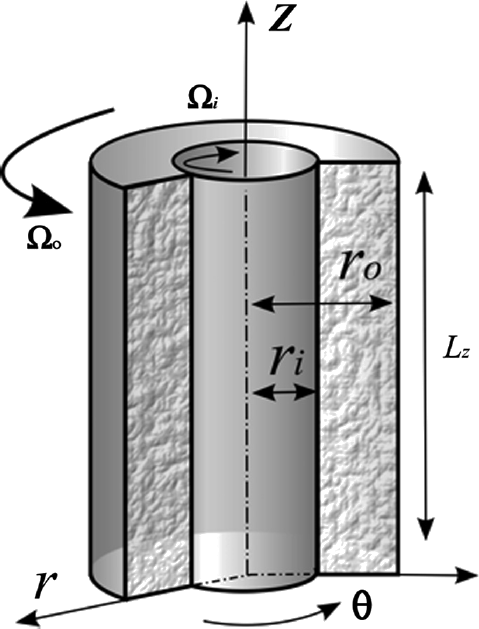
\includegraphics[width=1.00\linewidth]{figures/taylorCouette.png}
\caption{Schematic of the Taylor-Couette (TC) system in a cylindrical
co-ordinate frame work ($r, \theta, z$) and its relevant properties:
Radius of the inner/outer cylinder wall ($r_{i,o}$), height of the
computational domain ($L_z$), angular rotation speed of the inner/outer
cylinder walls ($\Omega_{i,o}$). Sketch taken from our CAF paper~\cite{Shi2015}.
% \df{Prepare a nicer sketch when we are done with everything else\dots}
}
\label{fig:tc}
\end{figure}
Rotating at least one of the cylinders causes a motion of the confined fluid;
A fluid-dynamical system well-known as Taylor-Couette (TC) flow. The so
generated fluid motion is governed by the incompressible Navier-Stokes equations
\begin{align}
\nabla\cdot\vec{u} = 0
\hspace{1em}\text{and}\hspace{1em}
\frac{\partial\vec{u}}{\partial t} + \vec{u}\cdot\nabla\vec{u} =
\frac{\nabla p^{\ast}}{\rho} + \nu\laplacian\vec{u}
\label{eq:nse}
\end{align}
which describe the conservation of mass and momentum in the system. Here, $t$
denotes the time, $p^{\ast}$ the hydrodynamic pressure, and $\vec{u}$ the velocity
vector, with its components $u_{r}$, $u_{\theta}$ and $u_{z}$ pointing along the
cylindrical coordinates in the radial ($r$), azimuthal ($\theta$) and axial ($z$)
direction.

\subsection{Control parameters and non-dimensional description}
\label{sec:controlParameters}

The TC geometry, as shown in figure~\ref{fig:tc}, can be fully characterised using
only two parameters. Its relative curvature is controlled by the radii ratio
$\eta=\sfrac{r_i}{r_o}$ of the inner and outer cylinder, whereas its relative height
is controlled by $\Gamma=\sfrac{L_z}{d}$, with $d=r_{o}-r_{i}$ being the gap-width
between the inner and outer cylinder wall. With the characteristic length scale set
to $d=1$, the inner and outer radius of the domain can be calculated as
\begin{align}
r_{i} = \frac{\eta}{1-\eta}
\quad\text{and}\quad
r_{o} = \frac{1}{1-\eta}
\end{align}
for any given $\eta$. For a fixed geometry, the flow between the cylinders can then
be fully characterised by only two additional parameters, namely the Reynolds number
\begin{align}
\Reynolds = \frac{u_{\text{ref}}\cdot d}{\nu}
=\frac{2}{1+\eta}\left(\Rei-\eta\Reo\right)
\end{align}
and the rotation number
\begin{align}
\Reom = \frac{2\omega_{\text{ref}}\cdot d}{u_{\text{ref}}} =
\left(1-\eta\right) \frac{\Rei+\Reo}{\Rei-\eta\Reo}
\text{,}
\end{align}
where $u_{\text{ref}}$ is a characteristic reference velocity and
$\omega_{\text{ref}}$ a characteristic angular velocity of the co-rotating reference
frame, see e.g. \cite{Dubrulle2005a} and \cite{Brauckmann2016}. The traditional Reynolds
numbers that measure the dimensionless velocity of the inner and outer cylinders in the
laboratory frame of reference, as e.g. used in the seminal experiments of Brandstäter
et al. \cite{Brandstater1983, Brandstater1987}, are given through
\begin{align}
\Rei = \frac{r_{i}\omega_{i}d}{\nu} = \frac{u_{i}d}{\nu}
\hspace{1em}\text{and}\hspace{1em}
\Reo = \frac{r_{o}\omega_{o}d}{\nu} = \frac{u_{o}d}{\nu}
\text{.}
\label{eq:reynoldsIO}
\end{align}
Henceforth, here and in the source code, all variables will be rendered dimensionless
using $d$, $\sfrac{d^2}{\nu}$, and $\sfrac{\nu^2}{d^2}$ as units for length, time,
and reduced pressure ($p=\sfrac{p^{\ast}}{\rho}$), respectively. Thus, we obtain a
non-dimensional form of the governing equations~(\ref{eq:nse}), in which \Rei and \Reo
appear only through a Dirichlet boundary condition for the velocity vector
\begin{align}
\vec{u}(r=r_{i,o}, \theta, z, t) =
\begin{bmatrix}
0 & \Reynolds_{i,o} & 0 
\end{bmatrix}^{\intercal}
\label{eq:noslipBC}
\end{align}
at the inner and outer wall of the cylinders. The unit for the velocity is already
implicitly defined through our choice for unit length ($d$) and unit time
($\sfrac{d^2}{\nu}$), and is thus given by $\sfrac{\nu}{d}$.




\section{Building the code}
\label{sec:buildingTheCode}

\subsection{Hardware prerequisites}
\label{sec:hardwarePrerequisites}

\nsc is written in modern \fortran and, over time, has been ported to all major
CPU-based high-performance computing (HPC) platforms. Amongst IBM Power,
BlueGene and \code{x86\_64} architectures -- including a few generations
of the prevalent Intel Xeon multi-core processors -- it has also been
ported to Xeon Phi (KnightsLanding), AMD EPYC (Naples) and ARMv8.1
(Marvell ThunderX2) platforms. Optimization for the NEC SX-Aurora vector
architecture is underway. The tutorials provided in section~\ref{sec:tutorials} of
this user guide were designed to run on standard laptops and small clusters.
\par
Additionally, we provide a GPU-accelerated (but basic) version of \nsc, which is
written in \c-\cuda and runs on a single GPU. In case you are interested in using
(or advancing) this version, you will need a \cuda-capable GPU device with compute
capability 2.0 (or superior) and support for double precision arithmetic.

\subsection{Software prerequisites}
\label{sec:softwarePrerequisites}

Building \nsc requires a Linux operating system, standard compilers and only
very few additional software libraries. All of them are commonly available as
high-quality, open source software packages or as vendor-optimised tool chains.
For the examples and tutorials (Section~\ref{sec:tutorials}) presented in this user
guide, we assume that you use a \code{bash} shell, although not necessarily 
required.

\subsubsection{Compiler}
\label{sec:compiler}

You need a modern \href{https://en.wikipedia.org/wiki/Fortran}{\fortran} compiler
which is \href{https://en.wikipedia.org/wiki/OpenMP}{\code{OpenMP3}} compliant.
Additionally, a corresponding \href{https://en.wikipedia.org/wiki/C_(programming_language)}{\code{C}}
compiler is necessary. \nsc has so far been tested with Intel's \code{ifort} and 
\code{icc} versions 12 through 15 as well as \code{PSXE2017} and \code{PSXE2018},
GNU's \code{GCC-4.7} to \code{GCC-4.9} and PGI's compilers version 14.
\par
Optionally, you will need a suitable version of NVIDIA's
\href{https://en.wikipedia.org/wiki/CUDA}{\cuda} toolkit in case you are interested
in working with the subsidiary GPU-accelerated version of our code.
Note, that in this case a suitable choice for the \cuda version highly depends on
the hardware you are going to use. The code runs on a single GPU and relies on the
\code{CcuFFT} library for computing Fourier transforms. Linear algebra is performed
using custon \code{CUDA} kernels. The GPU version of \nsc has so far been tested with
\cuda toolkit version from 8.0 to 10.1. Free software and further information can be found here:
\begin{itemize}
\item \url{https://gcc.gnu.org}
\item \url{https://developer.nvidia.com/cuda-toolkit}
\end{itemize}

\subsubsection{Message passing interface}
\label{sec:mpi}

You need an \href{https://en.wikipedia.org/wiki/Message_Passing_Interface}{\mpi} library which supports the thread-level \code{MPI\_THREAD\_SERIALIZED},
which means that the user code is multi-threaded, but calls to the \code{MPI} library are serialised. A fallback option for the minimum thread-level is implemented, which is supported by any \mpi implementation. \nsc has so far been tested with Intel's \code{MPI-4.1}, \code{5.0},
\code{5.1} as well as \code{IBM PE 1.3} and \code{1.5}. Free software and further information can be found here:
\begin{itemize}
\item \url{https://www.open-mpi.org}
\item \url{https://www.mpi-forum.org/docs/mpi-3.1/mpi31-report.pdf}
\end{itemize}

\subsubsection{Linear algebra}
\label{sec:linearAlgebra}

You need a serial \code{BLAS}/\code{LAPACK} library. \nsc has so far been tested with
Intel's \code{MKL-11.x}
% -> adapt \verb+LIBLA+ and/or point environment variable \verb+$MKL_ROOT+ to a MKL installation 
For free software and furthe information see:
\begin{itemize}
\item \url{https://en.wikipedia.org/wiki/LAPACK}
\item \url{http://www.openblas.net}
\item \url{http://math-atlas.sourceforge.net}
\item \url{http://www.netlib.org}
\end{itemize}

\subsubsection{Fastest Fourier transform in the west}
\label{sec:fftw}

You need a serial but fully thread-safe \code{FFTW3} installation
or equivalent. \nsc has so far been tested with \code{FFTW-3.3}
and also with the \code{FFTW} implementation which comes with
Intel's math kernel libraries \code{MKL-11.1} to \code{MKL-11.3}.
Earlier versions of \code{MKL} will likely fail.
%   -> point environment variable \verb+$FFTW_ROOT+ to a FFTW3 installation 
%   -> alternative: select  make FFTLIB=MKL (requires MKL 11.1 or later) 
For free software and further information see:
\begin{itemize}
\item \url{http://www.fftw.org}
\item \url{https://en.wikipedia.org/wiki/FFTW}
\item \url{https://en.wikipedia.org/wiki/Math_Kernel_Library}
\end{itemize}

\subsubsection{Hierarchical data format}
\label{sec:hdf5}

Optionally, you need an \code{MPI}-parallel \code{HDF5} library installation to
enjoy full flow field output in primitive variables (Section~\ref{sec:iohdf5})
which can be readily visualised using e.g. \paraview (Section~\ref{sec:paraview})
or \visit (Section~\ref{sec:visit}). \nsc has already been tested with
\code{HDF5-1.8.x} and \code{HDF5-1.10.0-patch1}. However, in case you don't need
\hdf output for now or encounter difficulties in providing a suitable \hdf
installation, you can ignore this software requirement and simply switch this
feature off (\code{HDF5IO=no}) when you compile the code
(Section~\ref{sec:compileTimeOptions}). 
The GPU version requires standard HDF5 libraries and provides an output
compatible with the \code{FORTRAN} code for visualisation.
Free software and further information can
be found here:
\begin{itemize}
\item \url{http://www.hdfgroup.org/HDF5}
\item \url{https://portal.hdfgroup.org/display/support}
\item \url{https://en.wikipedia.org/wiki/Hierarchical_Data_Format}
\end{itemize}
% -> point environment variable \verb+$HDF5_ROOT+ to an MPI-parallel HDF5 installation 

\subsubsection{Software modules}
\label{sec:softwareModules}

If you are planing to run \nsc on a supercomputer at a common national
high-performance computing centre (e.g. \href{https://www.lrz.de/english/}{LRZ}, 
\href{https://www.hlrs.de/home/}{HLRS}, 
\href{http://www.fz-juelich.de/ias/jsc/EN/Home/home_node.html}{JSC} or 
\href{https://www.hlrn.de/home/}{HLRN} in Germany), all of the above mentioned
software packages will most likely be readily available as user-loadable 
\href{http://modules.sourceforge.net/}{modules}. As a first step, you should make
yourself familiar with the system you are going to use and see
what software is already available. Some useful basic commands to start working
with environmental modules are listed in the following.
\begin{lstlisting}[language=bash]
feldmann@fsmcluster:~/$ module list
feldmann@fsmcluster:~/$ module avail
feldmann@fsmcluster:~/$ module avail 2>&1 | grep -i intel
feldmann@fsmcluster:~/$ module load moduleName
feldmann@fsmcluster:~/$ module switch moduleName
feldmann@fsmcluster:~/$ module purge
...
feldmann@fsmcluster:~/$ which mpiifort
feldmann@fsmcluster:~/$ mpiifort --version
\end{lstlisting}

\subsubsection{Self-build libraries}
\label{sec:selfBuildLibraries}

If you are, however, planing to run \nsc on your laptop, desktop, or local
institute cluster, you will most likely have to install some or all of the above
mentioned software packages yourself, before you can build and run \nsc. 
Regarding \mpi and the compilers, it is worth trying to install them using your 
favourite software package manager (\code{apt-get}, \code{rpm} and alike). For
the rest, it might be necessary to download the source files and 
build the libraries yourself. In appendix~\ref{app:selfBuildLibraries}, you will find detailed
examples of how to correctly configure and build some libraries (\code{zlib} and 
\hdf) for the use with \nsc on our local \code{fsmcluster} at the  
\href{https://www.zarm.uni-bremen.de/en/}{ZARM} institute. 
These examples can be used as a rough guideline to install all necessary software
packages on your target Linux system.

\subsection{Download the source files}
\label{sec:download}

Once you have checked that you have all the compilers and libraries installed
on your target system, you can proceed downloading the \nsc source files. Log
into the machine where you want to install and run \nsc. Make sure you are in
your home directory and create the \nsc working directory.
\begin{lstlisting}[language=bash]
feldmann@darkstar:~/$ cd $HOME
feldmann@darkstar:~/$ mkdir nsCouette
feldmann@darkstar:~/$ cd nsCouette
\end{lstlisting}
This is the place where you should put the source files. This is also the place, 
where we choose to put all the case directories -- one for each tutorial
(Section~\ref{sec:tutorials}) -- so that we have everything together in one place. Note,
however, that depending on the system you are working on, policy and quotas might
require you to store your simulation data (i.e. the case directories) in
designated file systems other than your home partition.
\par
You either got the source files as a \code{tar} archive file from one of the
authors or you can download the source files from our publicly available
\href{https://github.com/dfeldmann/nsCoutte}{\code{github}} repository.
In the first case, copy the archive into the working directory you just created
and unpack it.
\begin{lstlisting}[language=bash]
feldmann@darkstar:~/nsCouette$ tar xfvz nsCouette.tar.gz
feldmann@darkstar:~/nsCouette$ ls
nsCouette nsCouette.tar.gz
\end{lstlisting}
The latter option requires a working \code{git} installation, which is a
\href{https://git-scm.com/}{distributed version control system}. Most of
the time, \code{git} will either be readily available on your system or
it can be installed using your favourite software package manager.
\begin{lstlisting}[language=bash]
feldmann@darkstar:~/nsCouette$ sudo apt-get install git
...
feldmann@darkstar:~/nsCouette$ git clone https://github.com/dfeldmann/nsCouette
feldmann@darkstar:~/nsCouette$ cd nsCouette
feldmann@darkstar:~/nsCouette/nsCouette$ git checkout nsCouette-1.0
feldmann@darkstar:~/nsCouette/nsCouette$ git checkout nsCouette-gpu
feldmann@darkstar:~/nsCouette/nsCouette$ git checkout nsPipe-1.0
feldmann@darkstar:~/nsCouette/nsCouette$ git status
feldmann@darkstar:~/nsCouette/nsCouette$ git pull
\end{lstlisting}
Once you have \code{git} running, the \nsc source file remote
repository can than easily be cloned (downloaded) to your target
system with one single command. This first step has to be done
only once and by default you should be on the branch \code{nsCouette-1.0}.
But you can easily switch to other branches using the
\code{checkout} command to have access to the pipe flow variant
or the GPU-accelerated \cuda version. The
\code{git} commands \code{status} and \code{pull} will help you
to figure out on which branch you currently are and will get you
the latest changes (e.g. bug fixes or new features) from the remote
repository. A few more helpful hints on how to use \code{git} can
be found in appendix~\ref{app:git}.  

\subsection{Compile the code}
\label{sec:compile}

Once you have downloaded the source files (Section~\ref{sec:download}),
you can proceed building the executable. Go to the top-level directory
of the source files. Among other things, here you will find the following
files and directories, which are important to compile \nsc.
\begin{lstlisting}[language=bash]
feldmann@darkstar:~/nsCouette/nsCouette$ ls
...
ARCH/     scripts/    Makefile    nsCouette.f90   perfdummy.f90
mod_fdInit.f90  mod_inOut.f90  mod_timeStep.f90  mod_fftw.f90    mod_hdf5io.f90
mod_myMpi.f90   mod_vars.f90   mod_getcpu.f90 mod_nonlinear.f90  mod_params.f90
...
\end{lstlisting}
The source code is organised in twelve \fortran files (\code{.f90}), as
described in section~\ref{sec:codeStructures} in more detail. Among other things,
the directory \code{scripts} contains example files which will help you
to easily set-up the correct environment variables which are necessary for
building -- and also running -- the code. Have a look at them and make a
copy of one of the templates which appears closest to your platform/situation
and modify it accordingly using your favourite text editor (e.g. \code{vi}).
\begin{lstlisting}[language=bash]
feldmann@darkstar:~/nsCouette/nsCouette/scripts$ ls 
nsCouetteAtDarkstar.sh  nsCouetteAtFsm.sh  nsCouetteAtKonrad.sh  nsPipeAtKonrad.sh 
submit_loadl.sh  submit_sge.sh  submit_slurm.sh
feldmann@darkstar:~/nsCouette/nsCouette/scripts$ cp n*Darkstar.sh nsCouetteAtMyPlatform.sh
feldmann@darkstar:~/nsCouette/nsCouette/scripts$ vi nsCouetteMyPlatform.sh
\end{lstlisting}
By modifying we mean, that you should load the desired modules
(Section~\ref{sec:softwareModules}) and/or set all necessary
library path variables correctly (Section~\ref{sec:selfBuildLibraries}).
Also, you might find it convenient to create an alias in your
\code{.bashrc} so that you can easily load the correct environment
by simply typing \code{nsc} any time you log into your machine
or open a new terminal window. Note, that you have to load this
environment every time you want to (re-) compile the code and
also every time you want to run the executable (Section~\ref{sec:runningTheCode}).
\begin{lstlisting}[language=bash]
feldmann@darkstar:~$ vi .bashrc
...
alias nsc="source $HOME/nsCouette/nsCouette/scripts/nsCouetteAtDarkstar.sh"
...
feldmann@darkstar:~$ source .bashrc
feldmann@darkstar:~$ nsc
\end{lstlisting}


\subsubsection{Makefile settings}
\label{sec:makefile}

In general, the \code{Makefile} itself requires no editing by the user.
It is, however, advisable to have a look at it at some point to get an
idea of how \nsc is structured and build. Instead of modifying the
\code{Makefile}, all platform-specific settings should be fixed using
the architecture files. You can find a variety of working examples for
different systems in the respective directory. Have a look, copy the
template which appears closest to your platform/situation and modify it
accordingly using your favourite text editor (e.g. \code{vi}).
\begin{lstlisting}[language=bash]
feldmann@darkstar:~/nsCouette/nsCouette/ARCH$ ls
make.arch.darkstar   make.arch.gcc-openblas  make.arch.Supermuc
make.arch.fsm  make.arch.Hydra   make.arch.XC30_sisu-cray
make.arch.gcc-atlas  make.arch.intel-mkl  make.arch.XC30_sisu-intel
make.arch.gcc-essl   make.arch.KNL-intel  make.arch.xl-essl
make.arch.gcc-linux  make.arch.nec-aurora
make.arch.gcc-mkl make.arch.pgi-mkl
feldmann@darkstar:~/nsCouette/nsCouette/ARCH$ cp make.arch.darkstar make.arch.myPlatform
feldmann@darkstar:~/nsCouette/nsCouette/ARCH$ vi make.arch.myPlatform
\end{lstlisting}
By modifying we mean, that you should configure the correct compiler and libraries 
according to your environment and also specify the desired compiler options (e.g.
hardware specific optimisation flags). In case you use self-made libraries (see 
section~\ref{sec:selfBuildLibraries} and appendix~\ref{app:selfBuildLibraries}),
make sure to set all necessary path variables correctly (e.g. \code{LD\_LIBRARY\_PATH}).
Please consult your local IT support in case of problems. 
\par
If everything is configured correctly, the executable can be (re-)build in the usual way by
simply typing \code{make} and specifying the desired architecture file. It is recommended 
to always \code{clean} the build directory before each compilation. 
\begin{lstlisting}[language=bash]
feldmann@darkstar:~/nsCouette/nsCouette$ make ARCH=myPlatform clean
feldmann@darkstar:~/nsCouette/nsCouette$ make ARCH=myPlatform
...
feldmann@darkstar:~/nsCouette/nsCouette$ ls
ARCH/ darkstar/ myPlatform/ myPlatformGcc/ myPlatformIntel/
...
feldmann@darkstar:~/nsCouette/nsCouette$ ls darkstar/
nsCouette.x
...
\end{lstlisting}
If the code compiles correctly, a new sub directory is generated, it contains all the 
generated objects (\code{.o}) and modules (\code{.mod}) as well as the executable 
\code{nsCouette.x} itself. The subdirectory is named after the architecture file you 
specified (here e.g. \code{ARCH=myPlatform}). Specifying another architecture file, will
generate another subdirectory with another executable. This way you are able to easily 
manage different builds side by side. 

\subsubsection{Compile-time options}
\label{sec:compileTimeOptions}

Besides specifying the architecture file (Section~\ref{sec:makefile}),
the \code{make} command also takes a few other options which help you to
control the build process. The different options listed below can be
arbitrarily combined. They are meant to switch off \hdf flow field output
(Section~\ref{sec:iohdf5}), to include integrating the temperature for
thermal convection and heat transfer (Section~\ref{sec:thermalConvection}),
and to build the code in debug mode (i.e. tightest debug settings of the
compiler and no hardware specific optimisation). The respective default
value is the first choice in the angled brackets.
\begin{lstlisting}[language=bash]
feldmann@darkstar:~/nsCouette/nsCouette$ make ARCH=myPlatform HDF5IO=<yes|no>
feldmann@darkstar:~/nsCouette/nsCouette$ make ARCH=myPlatform CODE=<STD_CODE|TE_CODE>
feldmann@darkstar:~/nsCouette/nsCouette$ make ARCH=myPlatform DEBUG=<no|yes>
\end{lstlisting}



\section{Running the code}
\label{sec:runningTheCode}

Once you have compiled the executable (Section~\ref{sec:compile}), you
are almost ready to run a simulation. Create a case directory and make
sure that you have at least the executable and a parameter input file 
(Section~\ref{sec:parameterInputFile}) in that case directory.
\begin{lstlisting}[language=bash]
feldmann@darkstar:~/nsCouette/nsCouette$
feldmann@darkstar:~/nsCouette/nsCouette$ mkdir myCase01
feldmann@darkstar:~/nsCouette/nsCouette$ cp nscouette/myPlatform/nsCouette.x  myCase01/.
feldmann@darkstar:~/nsCouette/nsCouette$ cp nscouette/myPlatform/nsCouette.in myCase01/.
feldmann@darkstar:~/nsCouette/nsCouette$ cd myCase01
feldmann@darkstar:~/nsCouette/nsCouette/myCase01$ ls
nsCouette.in   nsCouette.x
feldmann@darkstar:~/nsCouette/nsCouette/myCase01$ ./nsCouette.x < nsCouette.in
\end{lstlisting}
Basically, the parameter input file is simply passed to the standard input
when you call the executable. A few detailed examples are described in the
tutorials (Section~\ref{sec:tutorials}).

\subsection{Parameter input file}
\label{sec:parameterInputFile}

In general, \nsc has to be build only once on a system and the executable
can be used for all your simulations within one research project. Most of
the settings and parameters to control the simulation can be specified at
run-time using a parameter input file. This file can have any name (here
\code{nsCouette.in}) and it is simply passed to the standard input when
calling the executable (here \code{nsCouette.x}). The parameter input
file should contain all of the following \fortran namelists. However, the
keywords within a namelist can appear in any order and individual keywords
can also be omitted if not needed.
\begin{lstlisting}[language=fortran]
&parameters_grid
m_r   = 32                   ! Radial points           => m_r      grid points
m_th  = 16                   ! Azimuthal Fourier modes => 2*m_th+1 grid points
m_z0  = 16                   ! Axial Fourier modes     => 2*m_z0+1 grid points
k_th0 = 6.0                  ! Fundamental wavenumber  => L_th = 2*pi/k_th0
k_z0  = 2.6179938779914944d0 ! Fundamental wavenumber  => L_z  = 2*pi/k_z0
eta   = 0.868d0              ! Radii aspect ratio
/

&parameters_physics
Re_i =   200.0d0           ! Inner cylinder Reynolds number
Re_o =  -200.0d0           ! Outer cylinder Reynolds number
Gr   =    50.0d0           ! Grashof number, Gr = Ra/Pr            [TE_CODE only]
Pr   =     0.71d0          ! Prandtl number                        [TE_CODE only]
gap  =     3.25d0          ! Gap size in cm                        [TE_CODE only]
gra  =   980.0d0           ! Gravitational acceleration in g/cm**3 [TE_CODE only]
nu   =     1.01d-2         ! Kinematic viscosity in cm**2 /s       [TE_CODE only]
/

&parameters_timestep
numsteps    = 10000        ! Number of timesteps to compute
variable_dt = T            ! Use a variable (T) or a constant (F) timestep size
init_dt     = 1.00d-5      ! Initial (T) or constant (F) size of timestep
maxdt       = 1.00d-2      ! Maximum allowed size of timestep (T)
Courant     = 0.25d+0      ! CFL safety factor
/

&parameters_output
fBase_ic = 'myCase01'   ! identifier for coeff_ (checkpoint) and fields_ (hdf5) files
dn_coeff = 2000         ! output interval [steps] for coeff (dn_coeff = -1 disables ouput)
dn_ke    = 100          ! output interval [steps] for energy
dn_vel   = 100          ! output interval [steps] for velocity
dn_Nu    = 100          ! output interval [steps] for Nusselt (torque)
dn_hdf5  = 1000         ! output interval [steps] for HDF5 output
dn_prbs   = 10          ! output interval [steps] for time series data at probe locations
prl_r(1)  = 0.20d0      ! radial probe locations (0 < r/d < 1)
prl_r(2)  = 0.50d0
prl_r(3)  = 0.80d0
prl_r(4)  = 0.20d0
prl_r(5)  = 0.50d0
prl_r(6)  = 0.80d0
prl_th(1) = 0.25d0      ! azimuthal probe locations (0 < th/L_th < 1)
prl_th(2) = 0.25d0
prl_th(3) = 0.25d0
prl_th(4) = 0.75d0
prl_th(5) = 0.75d0
prl_th(6) = 0.75d0
prl_z(1)  = 0.25d0      ! axial probe locations (0 < z/L_z < 1)
prl_z(2)  = 0.25d0
prl_z(3)  = 0.25d0
prl_z(4)  = 0.75d0
prl_z(5)  = 0.75d0
prl_z(6)  = 0.75d0
print_time_screen = 100 ! output interval [steps] for timestep info to stdout
/

&parameters_control
restart = 0             ! from scratch (0) or restrat from checkpoint file (1,2)
runtime = 86400         ! maximum wall-clock time for the job in seconds
/

&parameters_initialcondition
ic_tcbf = T ! Set Taylor-Couette base flow (T) or resting fluid (F), only when restart = 0
ic_temp = F ! Set temperature profile (T) or zero (F), only when restart = 0, only TE_CODE
ic_pert = T ! Add perturbation on top of base flow (T) or not (F), only when restart = 0
ic_p(1, :) = 4.0d-2, 0, 1 ! 1st perturbation: amplitude and wavevector (a1, k_th1, k_z1)
ic_p(2, :) = 6.0d-3, 1, 0 ! 2nd perturbation: amplitude and wavevector (a2, k_th2, k_z2)
ic_p(3, :) = 0.0d-0, 0, 0 ! 3rd perturbation: amplitude and wavevector (a3, k_th3, k_z3)
ic_p(4, :) = 0.0d-0, 0, 0 ! Add up to six user defined perturbations
/
\end{lstlisting}

\subsubsection{Control the time stepper}
\label{sec:controlTimeStepper}

The temporal integration scheme has been upgraded to a predictor-corrector
method, see also sec.~\ref{sec:timeStepper}. This enables a variable timestep
size ($\Delta t$), which is dynamically controlled during run time. This is
of particular advantage if the flow state is either suddenly modified
(applying disturbances, changing rotation rates etc.) or naturally undergoes
strong dynamics.
\par
The time stepper can be easily controlled on a user-level using the name list
\code{parameters \_timestep} in the parameter input file. Here, the number of
timesteps can be specified, which determines how many times the code runs
through the main time integration loop. Additionally, you can choose between
a user-specified constant $\Delta t$ and a variable $\Delta t$. If you chose
a variable timestep size by setting \code{variable\_dt=T}, then $\Delta t$ will 
be automatically updated every now and then according to the limits you can 
also specify in this name list --- the care-free package! In case
you start a simulation from scratch (\code{restart=0}) the dynamic adaptation
process begins with the value you specified at \code{init\_dt} in the parameter
file. However, in case you restart your simulation from an existing flow field
file (\code{restart=<1|2>}), then the \code{init\_dt} in the parameter file will
be ignored and the dynamic adaptation process resumes with the last value for
$\Delta t$ which was stored within the velocity file. If you, on the other hand,
chose a constant timestep size by setting \code{variable\_dt=F}, then $\Delta t$
will always be set to the value you specify for \code{init\_dt} in the parameter
and it will not change during the simulation. Further possibilities to control the
time stepper, which however require rebuilding the code, are described in
sec.~\ref{sec:timeStepper}.
\par
Usually, you run the transient phase of a simulation with \code{variable\_dt=T}
and observe the development of $\Delta t$. As soon as you have reached a statistically
steady state and want to calculate statistics or create output for movies and what not,
than you resume the simulation with a constant $\Delta t$, which you set to a nice even
value (\code{init\_dt}) which fits your needs and is slightly below the minimum
$\Delta t$ of what you observed during the transient phase.

\subsubsection{Setting boundary conditions}
\label{sec:boundaryConditions}

The boundary conditions (BC) in the two homogeneous directions ($\theta$ and $z$) are
periodic; basically for all flow field variables. The BC at the solid cylinder walls can be
controlled through he name list \code{parameters\_physics}. To model the impermeable
but rotating cylinder walls of Taylor-Couette set-up, we impose Dirichlet boundary
conditions for the velocity field. The two cross-stream velocity components ($u_r$ and
$u_z$) are set to zero everywhere at the walls. The streamwise velocity component
($u_{\theta}$) is set to \Rei and \Reo everywhere at the inner and outer cylinder wall,
respectively, which corresponds to the rotation speed of the respective wall, see
eq.~(\ref{eq:reynoldsIO}).
\par
For the heat transfer version of \nsc, additional Dirichlet BC are imposed for the
temperature field to model the isothermal cylinder walls. The temperature difference
between the inner and outer cylinder wall can be controlled by choosing the desired
Rayleigh number (i.e. setting values for the Grashof and the Prandtle number) in the
same name list.

\subsubsection{Choosing initial conditions}
\label{sec:initialConditions}

Integrating the Navier-Stokes equations forward in time is a typical initial
value problem. Each simulation run needs proper initial conditions for the
full three-dimensional velocity field $\vec{u}(r,\theta,z,t_0)$ and --
optionally -- also for the temperature field $T(r,\theta,z,t_0)$. Basically,
you have two options how to specify initial values for the flow field
variables, which can be controlled using the keyword \code{restart} in the
parameter name list \code{parameters\_control}.
\begin{itemize}
\item 
You can choose to generate initial conditions in the code itself
(\code{restart=0}). Starting from scratch requires no additional
files and data other than the executable itself (\code{nsCouette.x})
and a parameter input file (\code{nsCouette.in}). You can run a
simulation right away, as exemplarily shown in the first tutorial
in section~\ref{sec:tc0040}. However, there are a few different
options how to generate initial conditions, as described below, and
some more will be implemented in the future.
\item
Or you can choose to read initial conditions from an existing file
you have at hand (\code{restart=<1|2>}). This file has to be a Fourier
coefficient file in binary format (Section~\ref{sec:ioCoeff}), which
you might have from a similar simulation case or from a former run
of the same case. See section~\ref{sec:checkpoint} for details of
the checkpoint-restart mechanism.
\end{itemize}


You can chose to prescribe a resting fluid as initial condition by
setting \code{ic\_tcbf=F}. To prescribe the (Taylor)-Couette
analytical solution as base flow set \code{ic\_tcbf=T}. No matter
what the base flow is, you can disturb it by superimposing up to
six different perturbations by setting \code{ic\_pert=T} and than
defining an amplitude and wave number vector for each perturbation.
The perturbations are designed to fulfil the no slip boundary
condition at the solid walls and to be divergence free by construction.
Figure \ref{fig:ic} shows some useful examples of different initial
conditions at $\Rei=\num{50}$.
\begin{figure}
\begin{subfigure}{1.0\textwidth}
\centering
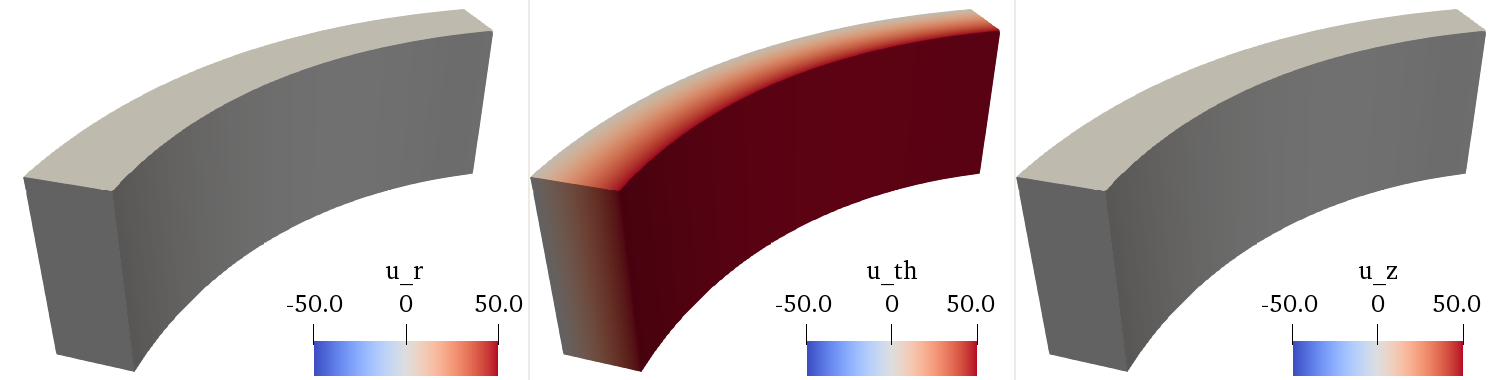
\includegraphics[width=0.8\textwidth]{figures/tc0039/icTaylorCouette.png}
\caption{Taylor-Couette analytical solution, no perturbation.}
\label{fig:tc0039icTayolorCouette}
\end{subfigure}
\vfill
\begin{subfigure}{1.0\textwidth}
\centering
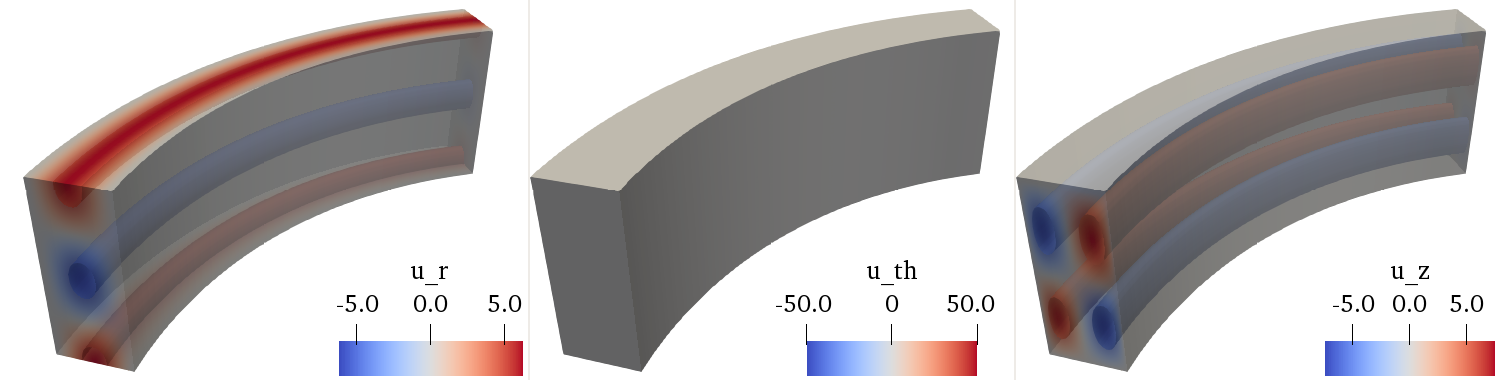
\includegraphics[width=0.8\textwidth]{figures/tc0039/icPerturb01.png}
\caption{Resting fluid, perturbed in mode $(l_{\theta,1}, n_{z,1})=(0,1)$
with amplitude $a_{1}=\num{e2}$.}
\label{fig:tc0039icPerturb01}
\end{subfigure}
\vfill
\begin{subfigure}{1.0\textwidth}
\centering
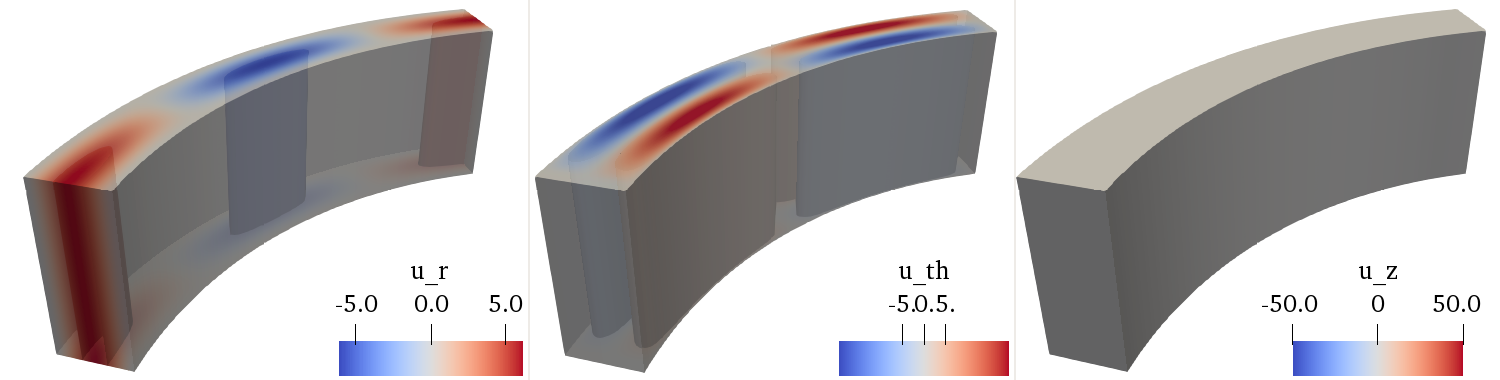
\includegraphics[width=0.8\textwidth]{figures/tc0039/icPerturb10.png}
\caption{Resting fluid, perturbed in mode $(l_{\theta,1}, n_{z,1})=(1,0)$
with amplitude $a_{1}=\num{e2}$.}
\label{fig:tc0039icPerturb10}
\end{subfigure}
\vfill
\begin{subfigure}{1.0\textwidth}
\centering
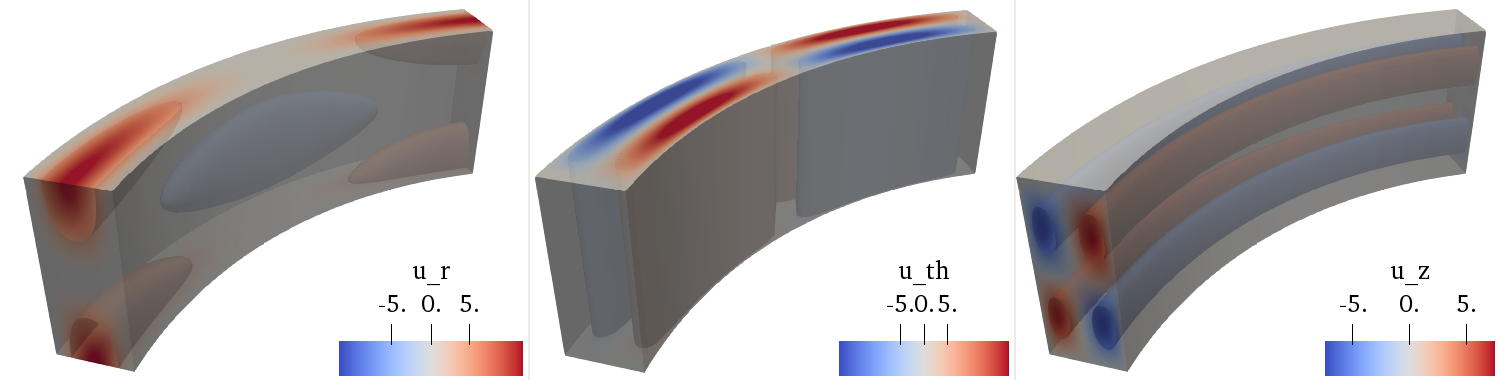
\includegraphics[width=0.8\textwidth]{figures/tc0039/icPerturb01and10.png}
\caption{Resting fluid, perturbed in modes $(0,1)$ and  $(1,0)$
with amplitudes $a_{1}=a_{2}=\num{e2}$.}
\label{fig:tc0039icPerturb01and10}
\end{subfigure}
\vfill
\begin{subfigure}{1.0\textwidth}
\centering
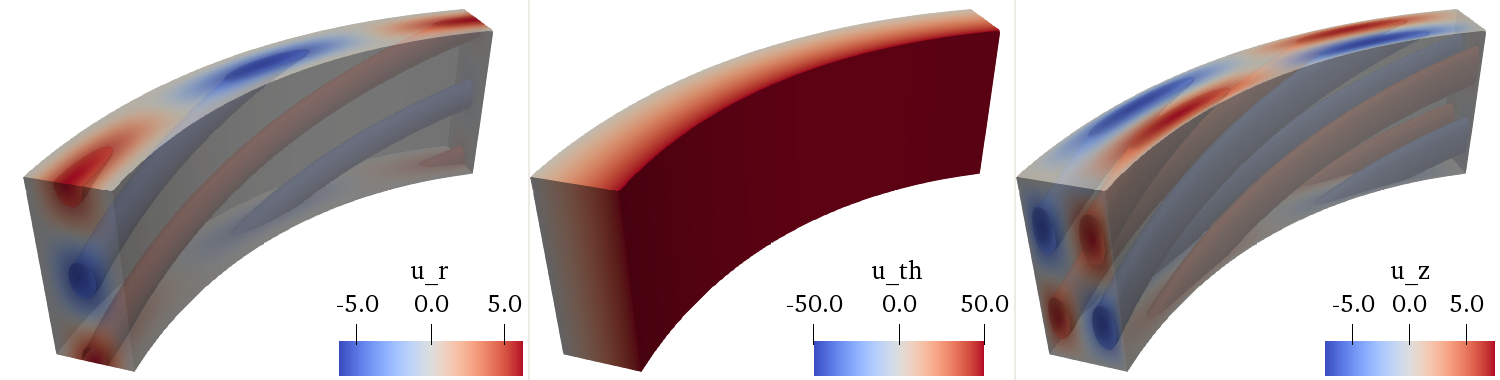
\includegraphics[width=0.8\textwidth]{figures/tc0039/icPerturb22.png}
\caption{Taylor-Couette base flow, perturbed in mode
$(l_{\theta,1}, n_{z,1})=(1,1)$ with amplitude $a_{1}=\num{e2}$.}
\label{fig:tc0039icPerturb22}
\end{subfigure}
\caption{Useful examples of different initial conditions at $\Rei=\num{50}$.
Shown are iso-contours (red/blue: $u_{\alpha}=\sfrac{\pm\Rei}{10}$) for all
three velocity components.}
\label{fig:ic}
\end{figure}
% Work in progress: Soon it will also be possible to read initial conditions from
% a \code{coeff*} file and add a perturbation on top by combining \code{restart=1}
% and \code{ic\_pert=T}.

\subsubsection{}

\subsection{On your laptop/desktop}
\label{sec:onYourLaptopDesktop}

Open a terminal. Go to your case directory. Copy the executable. And start the simulation with one MPI process.
\begin{lstlisting}[language=bash]
feldmann@darkstar:~$ cd nsCouette/tc0040
feldmann@darkstar:~/nsCouette/tc0040$ cp ../nscouette/darkstar/nsCouette.x .
feldmann@darkstar:~/nsCouette/tc0040$ ./nsCouette.x < nsCouette.in
\end{lstlisting}
To run \nsc with more than one MPI task, type
\begin{lstlisting}[language=bash]
feldmann@darkstar:~/nsCouette/tc0042$ mpiexec -np 32 ./nsCouette.x < nsCouette.in
\end{lstlisting}
Note, that the number of \mpi tasks can be freely selected at runtime with the only
restriction that it must evenly divide the number of radial grid points (parameter
\code{m\_r} in the input file). There is no such restriction regarding the total number
of Fourier modes (parameter \code{m\_f}, Appendix~\ref{sec:listOfParameters}). In these
cases, where the number of chosen \mpi tasks does not evenly divide \code{m\_f}, a few
dummy modes are automatically added. This causes a small imbalance and waste of
computational resources, which is reported at the beginning of the run, but gives
enormous flexibility in choosing spatial discretisation and degree of parallelisation.


\subsection{On a cluster}
\label{sec:onCluster}

Example batch submission scripts for the Sun Grid Engine (SGE) and
SLURM with Intel MPI, and IBM LoadLeveller with IBM MPI are provided
in the subdirectory \code{scripts}. Note that these scripts can serve only
as a rough guideline. They worked on a number of HPC systems but most
probably require some adaptation to a specific batch environment.


In this example setting a number of numsteps=10000 time steps would be
attempted to run, but the code would stop after a maximum runtime =
86400 seconds (24h) of (``wall-clock'') time. We have implemented an intrinsic
safety margin corresponding to the average number of seconds it takes to 2
timesteps.

If OpenMP is enabled (this is the default), set the 
environmental variable to specify the number of threads you would like to use. 
For example, specify
\begin{verbatim}
  export OMP_NUM_THREADS=4
  export OMP_PLACES=cores
  export OMP_SCHEDULE=static
  export OMP_STACKSIZE=256M
\end{verbatim}
if you want to use 4 OpenMP threads. The second line maps threads to
(physical) cores. The fourth line sets the stacksize, experiment with
larger or smaller values if unexpected SEGFAULTs occur or if the
memory per core is scarce, respectively.
These are just basic usage of MPI and OpenMP. 
For an advanced use of MPI and OpenMP (\textit{e.g.}, \verb+bash+ script) or in 
case of problems, please consult your local IT support.



\paragraph{Notes on runtime settings for hybrid MPI/OpenMP}
The most critical performance issue when running the code in hybrid mode (i.e.\
OpenMP enabled) can be an improper pinning of the MPI tasks and OpenMP threads to
the CPU cores. We suggest basic settings above based on the \verb+OMP_PLACES+
environment variable from the OpenMP standard, but different
compilers/runtimes and node architectures (NUMA, Hyperthreading,
\dots) might require specific settings. 
The actual mapping can be checked by examining the standard
output of \nsc, which, for an example with 16 nodes, 32 MPI
tasks (2 tasks per node) and 12 OpenMP threads per task should read
like this (the individual lines appear in random order):
\begin{small}
\begin{verbatim}
TASKS:  32 THREADS:12 THIS:   0  Host:nid01226   Cores:  0  1  2  3  4  5  6  7  8  9 10 11
TASKS:  32 THREADS:12 THIS:   1  Host:nid01226   Cores: 12 13 14 15 16 17 18 19 20 21 22 23
TASKS:  32 THREADS:12 THIS:   2  Host:nid01227   Cores:  0  1  2  3  4  5  6  7  8  9 10 11
TASKS:  32 THREADS:12 THIS:   3  Host:nid01227   Cores: 12 13 14 15 16 17 18 19 20 21 22 23
TASKS:  32 THREADS:12 THIS:   4  Host:nid01228   Cores:  0  1  2  3  4  5  6  7  8  9 10 11
TASKS:  32 THREADS:12 THIS:   5  Host:nid01228   Cores: 12 13 14 15 16 17 18 19 20 21 22 23
[...]
\end{verbatim}
\end{small}

Note, that the numbering scheme for the cores is due to some
low-level settings in the operating system and hence is highly machine
specific. Tools like \verb+cpuinfo+ (comes with Intel MPI) or 
\verb+likwid-topology+ (open source, see http://code.google.com/p/likwid/)
can be used to check the numbering scheme of a specific computer.

It is recommended to map at least one MPI task to each NUMA domain
(CPU socket) and specify \verb+OMP_NUM_THREADS+ to the number of
\emph{physical cores} (hyperthreading is not beneficial for
\nsc) of the CPU, divided by the number of  MPI tasks which we
map to this CPU. On contemporary HPC clusters with 2 Intel or AMD
CPUs per node, we typically use 2 MPI tasks per node and, for example 
set:
\begin{itemize}
\item \verb+OMP_NUM_THREADS=8+ (8-core CPUs, Intel Xeon E5-2670, \emph{SandyBridge})
\item \verb+OMP_NUM_THREADS=12+ (16-core CPUs, Intel Xeon E5-2698v3, \emph{Haswell})
\item \verb+OMP_NUM_THREADS=20+ (20-core CPUs, Intel Xeon Gold-6148, \emph{Skylake}) 
\item \dots
\end{itemize}
Note, however, that the OpenMP parallelism of the part of the code,
where the radial derivatives of the velocity are Fourier-transformed
to compute the nonlinear terms (performace label 'fft' in
mod\_nonlinear.f90), is limited by \verb+3*mp_r+ (or \verb+4*mp_r+, if the
\verb+make CODE=TE_CODE+ option is used), where $mp_r$ is the number of radial points
per MPI task. Thus, if the maximum number of MPI tasks is chosen for a
given number of radial points (and hence \verb+mp_r=1+), it is advisable to use 4 or 8  
MPI tasks per node on large multicore CPUs, and decrease
\verb+OMP_NUM_THREADS+ accordingly, in order not to waste resources.
A forthcoming release aims at alleviating this efficiency bottleneck by
supporting threaded FFTs.

\subsection{Output}
\label{sec:output}

\subsubsection{Time series data}
\label{sec:timeSeries}

If the program runs correctly, it immediately generates a set of data
files, which contain time series data of different quantities. These
files are updated continuously during the entire simulation run and
the sampling frequency for the time series output can be independently
specified using the keywords \code{dn\_ke}, \code{dn\_prbs} etc. in the
parameter input file, as detailed in section~\ref{sec:parameterInputFile}.
\begin{lstlisting}[language=bash]
feldmann@darkstar:~/nsCouette/tc0040$ ls
ke_mode  ke_total  probe01.dat  probe03.dat  probe05.dat  torque
ke_th    ke_z      probe02.dat  probe04.dat  probe06.dat  Nusselt
...
\end{lstlisting}
The first data column always contains the physical time in viscous units
($\sfrac{d^2}{\nu}$). See section~\ref{sec:controlParameters} for more
details on non-dimensionalisation. The other columns are the relevant
physical quantities like modal kinetic energy, integral torque, as well
as pressure, velocity and temperature at particular probe locations in the
flow field. The probe locations can be specified using the respective
keywords in the namelist \code{parameters\_output}, as detailed in
section~\ref{sec:parameterInputFile}. Since these files are simple
text files, the containing time series data can be easily read, plotted and
processed using any common editor, command line tool and plotting
programme (e.g. \code{gnuplot} or \code{xmgrace}). The tutorials in
section~\ref{sec:tutorials} provide further details and examples of how
to visualise and interpret the respective time series.

\subsubsection{Fourier space velocity field coefficients}
\label{sec:ioCoeff}

In \nsc the Fourier coefficients and optionally also the primitive variables are
independently dumped to individual files for each time step at user-specified 
output intervals. It also implements an easy-to-use checkpoint-restart mechanism 
based on the Fourier-coefficients for handling long-running DNS.
Checkpoint files are always written in binary MPI-IO format.
The binary coefficient files will be generated every \verb+dn_coeff+
timestep, according to the setting of the parameter in the input
file. Since in the example, we output the coefficient files every 2000 time steps within 
10000 total time steps, there will 5 coefficient files in total.
The name of the files will be like 
\begin{verbatim}
  coeff_DNS1.00002000
  coeff_DNS1.00004000
  ...  
  coeff_DNS1.00010000
\end{verbatim}
These files are the Fourier coefficients of the velocity field at one 
time step (``snapshot'') and can also be used as checkpoints to
continue a simulation (cf. Sect.~\ref{sec:checkpoint}). They can not be visualised straightforwardly but 
by some user-written post-processing utilities (\textit{e.g.}, using the library \verb+plplot+). 

\subsubsection{Physical space flow field data}
\label{sec:iohdf5}

 The primitive 
variables -- velocity ($u_r$, $u_{\theta}$, $u_{z}$), pressure ($p$) and 
optionally temperature ($T$) -- are written in \code{HDF5} format, along with 
metadata in a small \code{xdmf} file in order to facilitate analysis with common 
visualization tools like \code{ParaView} and \code{VisIt}. Both tools allow 
loading sequences of \code{xdmf} files produced by \nsc and enable the user to 
interactively perform comprehensive visual and quantitative analysis of the flow 
field. Sample scripts based on the \code{Python} interface of \code{VisIt}, as 
well as a custom-made \code{ParaView} filter for handling the cylindrical 
coordinate system % (VisIt has a built-in operator)
are distributed with \nsc. A detailed visualization tutorial is included in the
manual.


HDF5IO is switched on by default.
If HDF5IO is switched off (\verb+make ... HDF5IO=no+) only binary MPI-IO output will be written.
However, if you set \verb+HDF5IO=yes+ at the compilation time, 
the program will output \hdf-formatted files and corresponding
XDMF metadata files, as follows
\begin{verbatim}
  fields_DNS1_00001000.h5   fields_DNS1_00001000.xmf
  fields_DNS1_00002000.h5   fields_DNS1_00002000.xmf
  ...
  fields_DNS1_00010000.h5   fields_DNS1_00010000.xmf
\end{verbatim}
The \hdf format can be visualised with a lot of different visualisation software
tools. Here we discuss and shortly introduce two common open-source solutions;
i.e. \paraview (Section~\ref{sec:paraview}) and \visit (Section~\ref{sec:visit}). 

\subsection{Checkpoint-restart mechanism}
\label{sec:checkpoint}

On large HPC systems, the runtime of a single batch job is usually limited to something like
\SI{24}{\hour}. In order to enable long-running simulations, \nsc implements a semi-automatic
checkpoint-restart mechanism, where the initial conditions for the next run will be read from
a flow field file which was written at the end of the preceding run. Regardless of what you specify
for \code{dn\_coeff} in the parameter input file (Section~\ref{sec:parameterInputFile}), a
Fourier coefficient file (Section~\ref{sec:ioCoeff}) is written as a checkpoint at the very
end of any correctly terminated simulation run. Additionally, a small text file named \code{restart} is created, which is required to automatically continue the simulation in a next run. It contains the same information as the corresponding \code{*.info} file.
\par
By setting \code{restart=1} in the input file 
the simulation takes the information from the \verb+restart+ file and
uses the specified checkpoint file as the new initial condition,
rather than starting a new run (which corresponds the default setting \verb+restart=0+). 
The initial time for the new simulation run is that of the initial
condition and the time series data generated is appended to the existing
output files.
\par
A third initialization  option (\verb+restart=2+)
is also available, which allows to start the simulation
from a checkpoint file, but setting the time to zero and
creating new output files. The grid size of the continued simulation
can be modified by adapting the corresponding parameters in
the \verb+input_nsCouette+ file, but m\_r
must remain to be divisible by the number of processors. Writing of
checkpoints can be disabled by setting \verb+dn_coeff = -1+ in the input file.
%
Note, that the \verb+restart+ file is only written if a run has
finished successfully. If, on the contrary, the run terminates prematurely (e.g.
due to a hardware issue, or a numerical or code-specific problem),  
the last valid coefficient file can serve a checkpoint for restarting
the run. In such a case, the \verb+restart+ file has to be created
manually, simply by copying the corresponding \verb+coeff_ .info+
file. 

The checkpoint-restart mechanism allows submitting a chain of (many)
individual jobs to a batch system at once and thus facilitates handling of long-running
simulations with \nsc. Basic functionalities of the batch system (e.g.
options \verb+-hold_jid+ for SGE or \verb+--dependency+ for SLURM) can be 
used to express the chain-type dependency of the individual jobs.








\section{Post-processing}

\subsection{Visualisation with \texttt{\textbf{ParaView}}}
\label{sec:paraview}
To visualise and analyse instantaneous flow field data with the open source
software tool \code{ParaView}, see fig.~\ref{fig:paraViewFlowField}, just go
through the introductory steps below and follow our tutorials in section~\ref{sec:tutorials}.
\begin{figure}[htb]
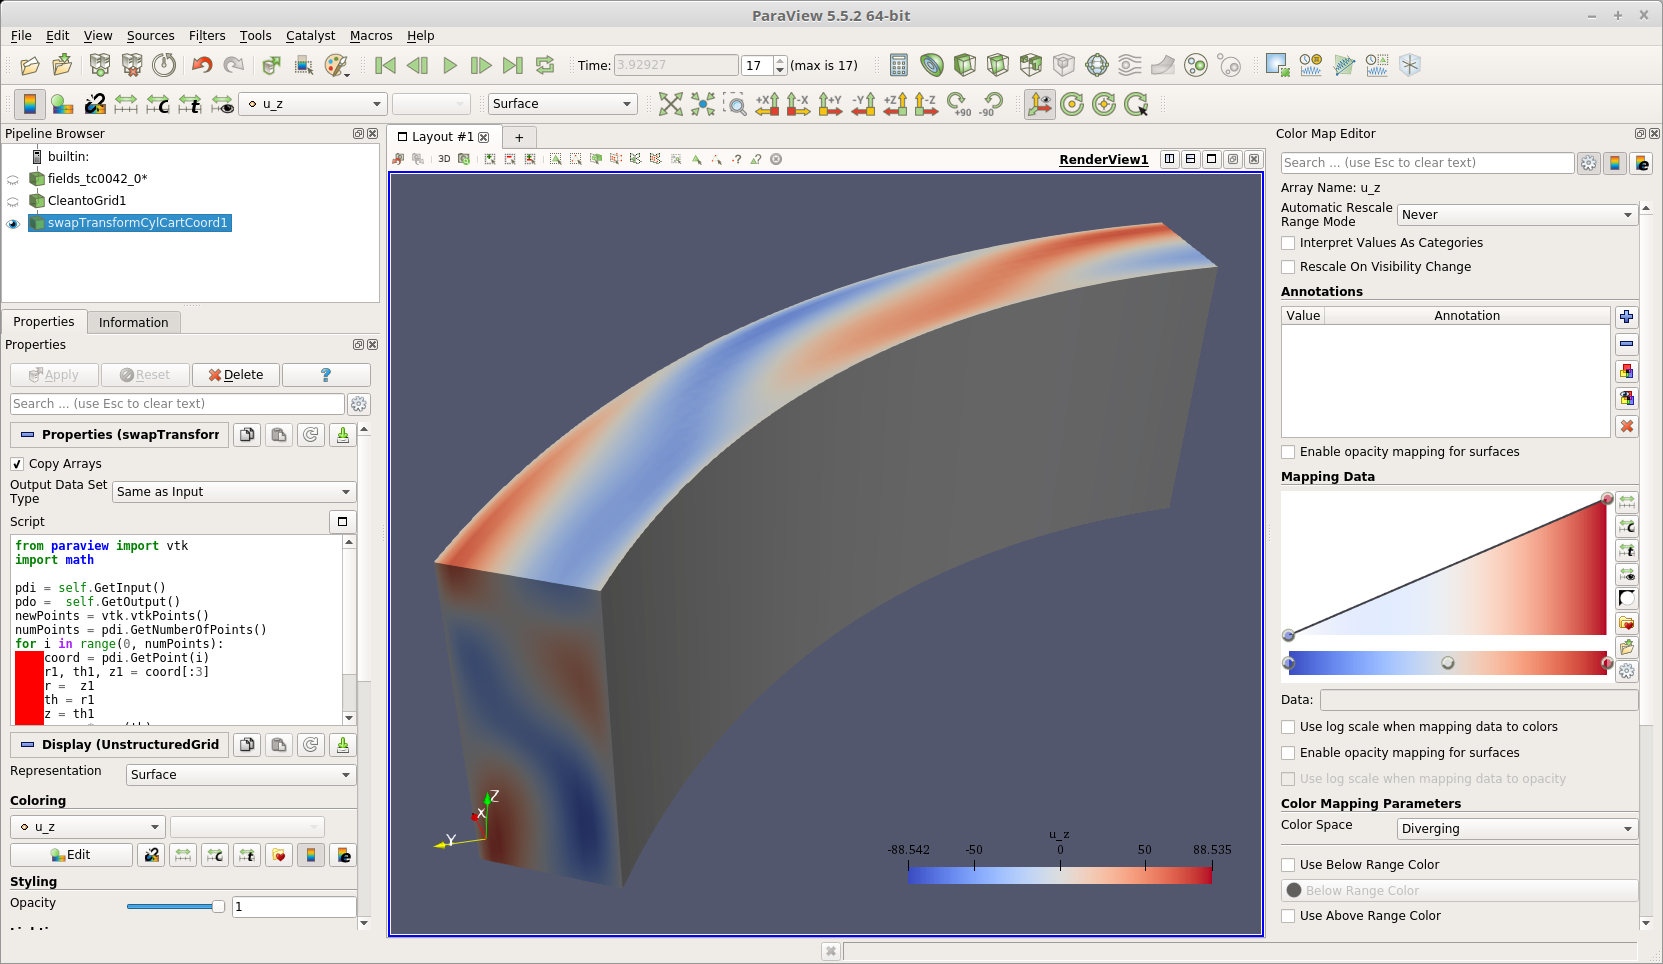
\includegraphics[width=1.00\linewidth]{figures/paraViewFlowField.png}
\caption{Screenshot of the \code{ParaView} GUI and the first basic steps to
visualise and analyse the \code{HDF5} flow field output from \nsc. Follow our
tutorials in section~\ref{sec:tutorials} for further details.}
\label{fig:paraViewFlowField}
\end{figure}
The tutorials also provide a few ready-to-use state files (\code{*.pvsm})
to start with. Note, however, that this is just a collection of very
basic quick-start recipes. For more information, please consult the
\href{https://www.paraview.org/Wiki/The_ParaView_Tutorial}{official documentation}
\cite{Moreland2018} and the pertinent online discussion forums.

\paragraph{Preparation}
\begin{itemize}
\item
Download a recent pre-compiled version from the official web page
\url{www.paraview.org} and follow the instructions to install and
run it. Or download the source files and build it yourself.
\item
Once you have \code{ParaView} running, you need to load a  costum-made
\code{python}-filter, which comes with \nsc. This filter can be used to
perform a coordinate transformation for every state file you load into
\code{ParaView}. This is a crucial step for correct three-dimensional
rendering of the flow field, since \code{ParaView} only knows Cartesian
coordinates ($x, y, z$), whereas the flow field data in the \code{HDF5}
output files is defined in a cylindrical coordinate system($r, z, \theta$),
see section~\ref{sec:}. To add the  costum filter to the list of known filters
do the following:
\begin{enumerate}
\item Launch \paraview
\item Chose from the menu \code{Tools} $\to$ \code{Manage custom filters}
\item Press \code{Import} in the upcoming window
\item Browse to \code{\$HOME/nsCouette/nsCouette/visualisation}
\item Select the file \code{swapTransformCylCartCoord.cpd}
\item Press \code{close}
\end{enumerate}
\end{itemize}
Now the filter is known to \paraview and can be used any time you
open this installation. To perform a coordinate transformation choose
\code{Filters $\to$ Alphabetical $\to$ swapTransformCylCartCoord}
from the menu.

\paragraph{Loading flow field data}
\begin{itemize}
\item
Once \paraview is installed and the transformation filter has been successfully
added, you can begin loading flow field data. You should go to the case
directory where you have stored the \hdf output files (here one of the first
tutorial cases section~\ref{sec:tc0042})
\begin{lstlisting}[language=bash]
feldmann@darkstar:~/$ cd nsCouette/tc0042
feldmann@darkstar:~/nsCouette/tc0042$ paraview &
\end{lstlisting}
and start \paraview.
\item
Once the \paraview main window has appeared (something like in
fig.~\ref{fig:paraViewFlowField}), chose from the menu \code{File $\to$ Open}
or click on the yellow folder icon in the top left corner to open the file
selection dialogue.
\begin{figure}[htb]
\centering
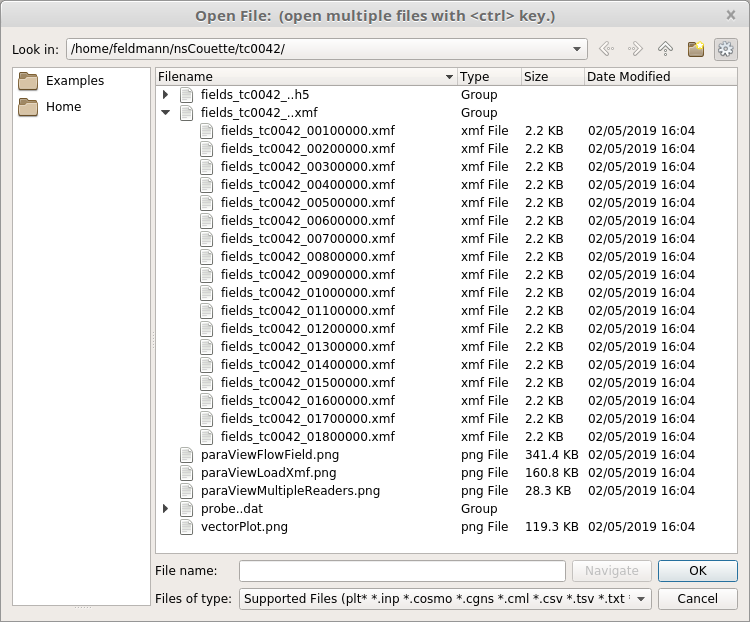
\includegraphics[height=0.42\linewidth]{figures/paraViewLoadXmf.png}\hfill
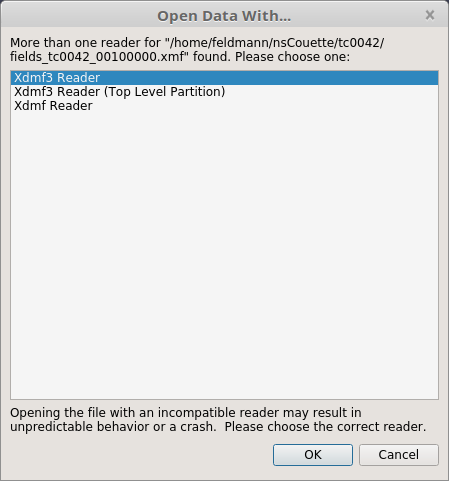
\includegraphics[height=0.42\linewidth]{figures/paraViewMultipleReaders.png}
\caption{Screenshot of the file open dialogue window (left) where you
can select the \code{xmf} files, which act as a reader or interface
through which \code{ParaView} access the flow field data contained in
the \hdf files. If there is more than one \code{xmf} reader, chose the
first on in the appearing dialogue window (right).}
\label{fig:paraViewFlowFieldLoadXmf}
\end{figure}
There you will see a list of the available \hdf files and the corresponding
\code{xmf} files as shown in figure~\ref{fig:paraViewFlowFieldLoadXmf}. The
\code{xmf} files are simple text files, which contain meta data about the
content of the \hdf container. The \code{xmf} files act as a reader or interface
through which \paraview access the data in the \hdf container. Select one single
or a group of several \code{xmf} files and press \code{OK}. Note, that all files
with the same base name are automatically grouped. So if there are many flow
field files in this directory, you can easily load the entire time series of
snapshots by selecting the group instead of a single \code{xmf} file. Note,
however, that loading a large number of snapshots might take very long for large
simulations!
\item
If a new dialogue window appears (fig.~\ref{fig:paraViewFlowFieldLoadXmf}
right) after selecting snapshots and pressing \code{OK}, then select the
option \code{Xdmf3 Reader}; but not \code{Xdmf3 Reader (Top Level Partition)}
or anything else. Otherwise ignore this step.
\item
Now press \code{Apply} in the main \paraview window to actually load the selected snapshots.
Note, that, since \paraview is designed to deal with large data sets, no action or data
manipulation takes actually place until you finally hit the \code{Apply} button.
\item
Note, that data extraction, manipulation and plotting in \paraview is accomplished
through so-called filters. You find a complete list of all available filters by
choosing \code{Filters $\to$ Alphabetical} from the menu. The pipe line browser
on the left shows all loaded data sets and all filters applied to it as individual
objects or instants in an hierarchical order. Always make sure that you select/highlight
the correct instant to which you want to apply the next filter operation.
\item
Once the data set has been loaded, you should first apply the following
two filters in exactly this order:
\begin{enumerate}
\item
Select \code{Filters $\to$ Alphabetical $\to$ Clean to Grid} from the menu
and than hit the \code{Apply} button.
\item
Select \code{Filters $\to$ Alphabetical $\to$ swapTransformCylCartCoord} from
the menu and than hit the \code{Apply} button to perform the transformation
from cylindrical to Cartesian coordinates.
\end{enumerate}
\item Now recenter the view by clicking the \code{Zoom to data} button to
obtain something similar to what is shown figure~\ref{fig:paraViewFlowField}.
\end{itemize}

\paragraph{Visualise flow field data}
\begin{itemize}
\item
Choose the quantity you are interested in. By default, this
might be the pressure $p$. To get something similar as shown
in figure~\ref{fig:paraViewFlowField}, select the e.g. the
axial velocity component $u_z$.
\item
If you have loaded more than one snapshot, you can simply hit
the green \code{Play} button to show a movie representation of
how the flow field changes with time. Note, that this process
might be very slow in case of large simulations.
\item
To extract iso-surfaces for different velocity components, as
shown for example in figure~\ref{fig:tc0041vectorPlot}, select
the instant named \code{swapTransformCylCartCoord} in the pipe
line browser, choose \code{Filters $\to$ Alphabetical $\to$
Contour} from the menu and hit \code{Apply}. Select the velocity
component you are interested in and modify the the contour levels
in the properties panel directly below the pipe line browser.
\item
To create a vector representation of the cross-stream velocity
components as for example in figure~\ref{fig:tc0041vectorPlot},
use the \code{Glyph} filter as exemplarily shown in the \paraview
state file \code{vectorPlot.pvsm} which comes with the second
tutorial described in section~\ref{sec:tc0041}.
\end{itemize}







\subsection{Visualisation using \visit}
\label{sec:visit}
As an alternative to \paraview (section~\ref{sec:paraview}), you can also use
the open source software \visit (fig.~\ref{fig:visit}), to visualise and
analyse the instantaneous flow field snapshots generated with \nsc.
\begin{figure}[htb]
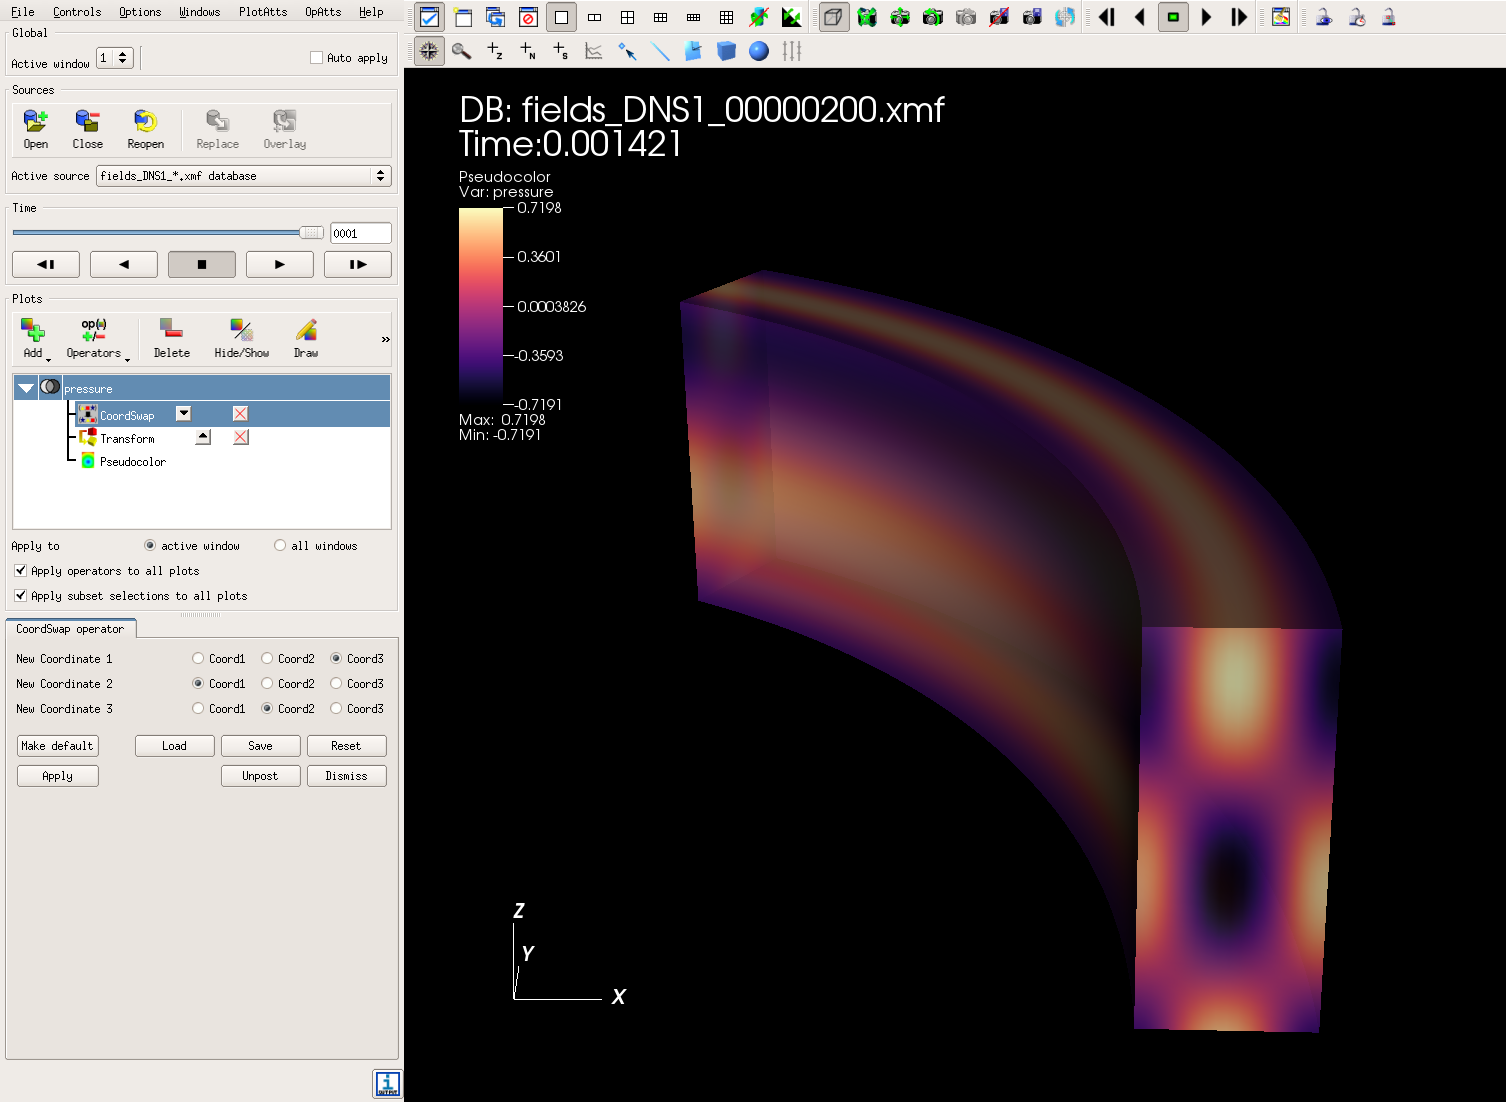
\includegraphics[width=1.00\linewidth]{figures/visit.png}
\caption{A screenshot of the \code{GUI} of \visit showing a basic example
of a pseudo-colour representation of the instantaneous pressure field in
a small computational domain similar to the set-up used in the first
tutorial in section~\ref{sec:tc0040}.}
\label{fig:visit}
\end{figure}
The following basic steps will give you a good starting point to learn
how to read the \hdf files and how to render the containing flow field
data.
\begin{itemize}
\item Download and install the software from the \href{https://wci.llnl.gov/simulation/computer-codes/visit}{official webpage}.
\item Move all the \code{.h5} and \code{.xmf} files to one directory (\code{DIR\_HDF5}) of your choice.
\item Go there and start \visit. A GUI window will pop up to select/open files.
\item Enter the path to \code{DIR\_HDF5}.
\item Select the \code{.xmf} files and press the \code{OK} button.
\item Two GUI windows will appear: The \visit main window (control panel) and the Vis window (white blank).
\item Press the \code{Add} button in the middle of the main window. From the
pull-down menu select the type of you want to plot, \textit{e.g.}, ``contour'' or ``pseudocolor'';
  \item  \textbf{Important step:} Add two operators one after another on the plot by clicking on the ``Operators'' next to the ``Add'' button. 
 Select in the pulldown menu ``CoordinateSwap'' to change our file coordinates $(\theta,z,r)$ to $(r,\theta,z)$ 
 and ``Transform'' to change our coordinate system from
 cylindrical to cartesian (cf. Fig.~\ref{fig:VisIt}); 
  \item  Click on ``OpAtts'' on the top toolbars in the Main window and change the operator attributes according to the above specifications.
  \item  Click on ``Draw'' and you have the plot in the right Vis window (for large file, it takes time!);
  \item  Play with the plot and carefully observe the change after each operation;
\end{itemize} 

\section{About the code}
\label{sec:aboutTheCode}

In this section, the code is further documented on a programming level;
i.e. structure, data types, variables, parallelisation etc. Additionally,
some details on selected methodological aspects are outlined. Further
technical documentation of the source code -- auto-generated with the
\code{FORD} tool -- can be found
\href{http://mjr.pages.mpcdf.de/nscouette/ford-doc/}{here}.

\subsection{Structure of the source code}
\label{sec:codeStructures}

The source code comprises only a few thousand lines of code, which are structured in
a minimum set of twelve basic source files -- including a \code{Makefile}. The different
parts of the code are thematically structured into separate files and \fortran modules
according to the following summary.
\begin{lstlisting}[language=bash]
feldmann@darkstar:~/nsCouette/nsCouette$ ls
...
Makefile   # Script file to compile the code
nsCouette.f90 # Main routine: Initialisation, time-stepping, finalisation
mod_params.f90   # All parameters and constants
mod_vars.f90  # Definition of all (derived) variables
mod_myMpi.f90 # MPI-related subroutines: windows, derived data types, etc.
mod_fftw.f90  # Subroutines related to fast Fourier transforms
mod_fdInit.f90   # Finite differences matrices for 1st and 2nd radial derivatives
mod_nonlinear.f90   # Subroutine to compute the nonlinear advection term (pseudo-spectral) 
mod_timeStep.f90 # The predictor-corrector time-stepper
mod_inOut.f90 # Messy collection of input, output, base flow, initial conditions
mod_hdf5io.f90   # HDF5 output of primitive flow field variables
mod_getcpu.f90   # Mapping of the CPU. This module cannot be included.
...
\end{lstlisting}

\subsection{Programme flow chart}
\label{sec:programmeFlowChart}

Basically speaking, the programme flow of \nsc is as follows.
\begin{enumerate}
\item Initialisation phase: \mpi, read parameter file (section~\ref{sec:parameterInputFile}), set initial conditions (section~\ref{sec:initialConditions}) 
\item Time-stepping: linear sub-step computation and nonlinear pseudo-computation)
\item Finalising phase: \mpi, checkpoint output (section~\ref{sec:})
\end{enumerate}


\subsection{Constants \& variables}
All constants are specified in \verb+mod_params.f90+, while all variables are given 
in \verb+mod_vars.f90+. The data type are mostly specified with \verb+KIND=4 or 8+, 
indicating single or double precision. The derived data types in \verb+mod_vars.f90+ 
are \verb+phys+ for variables in physical field, \verb+spec+ for variables in Fourier
 space and \verb+vec_mpi+ for vector variables in each MPI sub-domain. The type 
\verb+phys+ and \verb+spec+ contains all physically relevant quantities, \textbf{u} and p. 
The array of type \verb+vec_mpi+ is mainly used in the node-independent calculation and 
the data is arranged such that \verb+mp_f+ is a map of the couple 
\verb+(m_th,m_z/np)+. The distribution of the whole array \verb+(m_th,m_z)+ into each MPI task 
is according to the Fig.2 in our CAF paper~\cite{Shi2015}. 

\subsection{Temporal discretisation}
\label{sec:timeStepper}

Since the publication of our CAF paper~\cite{Shi2015}, quite some changes have been
implemented to \nsc to further improve its usability and performance. Notable among
these is the implementation of a new time-stepper. The governing equations are now
integrated forward in time using a predictor-corrector algorithm, which allows to
significantly increase the computational time step size $\Delta t$ in the simulation.
The ideas for this time-stepper were borrowed from the \opf project; an open source
code for pipe flow simulations developed by Ashley Willis~\cite{Willis2017}. A
comprehensive description can be found on Ashley's web page, while the basic steps
of our implementation are outlined in the following.
\begin{itemize}

\item
In the predictor step the equations are solved explicitly to obtain a rough
approximation of the velocity field $u_1^{q+1}$. If the matrices containing
the linear and non-linear terms are denoted as $L$ and $N$ respectively, the
predictor step can be written as
\begin{align*}
\nabla P_1^{q+1} & = \nabla\cdot(Lu^q+N^q)\\
\left(\frac{1}{\delta t} - c\nabla^2\right) u_1^{q+1} & =
N^q + \left(\frac{1}{\delta t}-(1-c)\nabla^2\right) u^{q} - \nabla P_1^{q+1}
\end{align*}

\item
The velocity computed in the predictor step ($u_1^{q+1}$) is then refined in
multiple corrector steps, until a certain tolerance is reached. The iteration
for the corrector step is given by
\begin{align*}
\nabla P_{j+1}^{q+1} & = \nabla\cdot\left(Lu^q+N_j^{q+1}\right)\\
\left(\frac{1}{\delta t}-c \nabla^2\right) u_{j+1}^{q+1} & =
c N_j^{q+1} + \left(1-c\right)N^q + \left( \frac{1}{\delta t} -
\left(1-c \right) \nabla^2 \right) u^{q} - \nabla P_{j+1}^{q+1}
\end{align*}
and the tolerance is set to \code{tolerance\_dterr = 5E-5} by default. If
necessary, it can easily by changed by modifying the file \code{mod\_param.f90},
see section~\ref{sec:}

  

\item The coefficient $c$ (d\_implicit) defines the implicitness of the method and can be specified
  in mod\_params.f90. Note that the temporal scheme is second-order if c=0.5.

\item The boundary conditions are imposed through influence matrices which are 
  computed at a pre-processing stage.


  \item The user can choose between fix or variable time-step size. In the latter case $\delta t$ is computed as
  \begin{equation}
 \delta t = C min (\nabla / |v|),
  \end{equation}
  
  where $C$ is the Courant number
  

\end{itemize}

\subsection{Feature for thermal convection}
\label{sec:thermalConvection}

You can easily switch to the optional temperature version of \nsc by simply
setting the external variable \code{CODE=TE\_CODE} when building the code.
Note, that the standard version of \nsc~-- i.e. without the additional
temperature equation -- is set by default (\code{CODE=STD\_CODE}), see also
section~\ref{sec:compileTimeOptions}.
\begin{lstlisting}[language=bash]
feldmann@darkstar:~/nsCouette/nsCouette$ make ARCH=myPlatform clean
feldmann@darkstar:~/nsCouette/nsCouette$ make ARCH=myPlatform HDF5IO=no CODE=TE_CODE
\end{lstlisting}
\par
The equation for the temperature ($T$) is coupled to the Navier--Stokes
equations by considering a Boussinesq-like approximation that includes
centrifugal buoyancy effects. Details about the dimensionless governing
equations and the Boussinesq-like approximation are documented in Lopez
et al.~\cite{Lopez2013}. Now, the code produces additional output. For
details also see section~\ref{sec:output}). The file \code{Nusselt}
contains time series of the normalised heat transfer at the inner and
outer cylinders walls and the file \code{Temp\_energy} contains time
series of the modal energy related to the temperature field. Time series
of the temperature at the some user specified probe locations do now
appear in the files \code{probes*.dat}. The snapshot flow field files
(\code{coeff\_*} and \code{fields*.h5}) now also contain full information
about the instantaneous temperature field.
\par
In the provided version of \nsc, the flow is stratified radially by
heating the inner cylinder and cooling the outer cylinder, i.e. a
negative radial temperature gradient $\sfrac{\partial T}{\partial r}$.

\subsubsection{How to modify the source code}

The sense of the temperature gradient can be easily modified by inverting
the boundary conditions for the temperature in the file \code{mod\_timeStep.f90}
and modifying the temperature and axial velocity of the base flow accordingly
in the \code{subroutine base\_flow} contained in the file \code{mod\_InOut.f90}.
\begin{lstlisting}[language=Fortran]
! Boundary conditions for mode 0 (prescribed temperature at the cylinders)  
if (abs(fk_mp%th(1,k)) <= epsilon .and. abs(fk_mp%z(1,k)) <= epsilon) then  
 rhs_p(1)   = dcmplx( 0.5d0, 0d0) 
 rhs_p(m_r) = dcmplx(-0.5d0, 0d0) 
end if
\end{lstlisting}




\section{Tutorials}
\label{sec:tutorials}

\subsection{Prerequisites}
\begin{itemize}
\item
Get a recent \code{gnuplot} installation to quickly inspect the time series output
interactively and to easily produce some decent line plots using the \code{*.gpl}
script files, which come with this tutorials. The scripts provided here were
generated and tested using version \code{5.0}. In appendix~\ref{app:}
you can find a sample instruction which will help you to install a recent version.
\begin{lstlisting}[language=bash]
feldmann@darkstar:~/nsCouette$ gnuplot --version
gnuplot 5.0 patchlevel 3
\end{lstlisting}
\item
For more advanced plotting and data analysis a recent \code{Python} installation can be
quite helpful. Some of this tutorials come with a few basic \code{*.py} script files
which can be used as a starting point for your further work.
\item
For three-dimensional flow field visualisation we recommend you to install \code{ParaView}
(Section~\ref{sec:paraview}) or \code{VisIt} (Section~\ref{sec:visit}).
\item
A proper \LaTeX~installation might also be useful e.g. to compile this manual or to convert
the \code{*.eps} output from \code{gnuplot} to proper \code{*.pdf} figures.
\end{itemize}

\subsection{Laminar Taylor-Couette flow in the stable regime}
\label{sec:tc0040}
To start off, we will first run a simulation of Taylor-Couette flow in the 
stable regime, i.e. at a very low Reynolds number. This allows us to perform our 
first DNS on a regular laptop in less than a minute. Moreover, we can readily 
compare the results to what we expect from theory. Go to your working directory, 
copy the first Taylor-Couette tutorial case from the repository and inspect the 
parameter input file (\code{nsCouette.in}) using your favourite  text editor
(e.g. \code{vi}, \code{emacs}, \code{kate}, \code{gedit} and such).
\begin{lstlisting}[language=bash]
feldmann@darkstar:~$ cd ~/nsCouette
feldmann@darkstar:~/nsCouette$ cp -r ../nscouette/tutorials/tc0040 .
feldmann@darkstar:~/nsCouette$ cd tc0040
feldmann@darkstar:~/nsCouette/tc0040$ vi nsCouette.in
\end{lstlisting}
We choose to keep the outer cylinder wall stationary by setting $\Reo=0$ and further
choose a very low rotation speed of the inner cylinder by setting $\Rei=50$. The
corresponding part in the input file \code{nsCouette.in} looks like this.
\begin{lstlisting}[language=Fortran]
&parameters_physics
Re_i = 50.0d0   ! inner cylinder Reynolds number
Re_o =  0.0d0   ! outer cylinder Reynolds number
/
\end{lstlisting}
All the other parameters in this namelist (\code{parameter\_physics}) are
irrelevant for our first tutorials. They will be discussed later in
section~\ref{sec:tc0073}, when we turn to thermal convection. See also
section~\ref{sec:parameterInputFile} and \ref{sec:listOfParameters} for
an exhaustive description of the parameter input file. Due to this very
small Reynolds number, a very coarse spatial resolution should be sufficient
to produce accurate results. Here, we choose $M=16$ radial grid points in
physical space and $N=L=4$ Fourier modes in azimuthal ($\theta$) and axial
($z$) direction, respectively. The corresponding entries in the namelist
\code{paramters\_grid} are shown here.
\begin{lstlisting}[language=Fortran]
&parameters_grid
m_r  = 16            ! M grid radial points
m_th =  4            ! N azimuthal Fourier modes
m_z0 =  4            ! L axial Fourier modes
/
\end{lstlisting}
This choice corresponds to a total of $n_r \times n_\theta \times n_z=M \times 
(2N+1) \times (2L+1) = \num{16} \times \num{9} \times \num{9}$ significant 
physical grid points, while the nonlinear terms are actually evaluated on $M 
\times (3N+1) \times (3L+1) = \num{16} \times \num{13} \times \num{13}$ physical 
grid points for dealiasing purposes. For further details, definitions and 
notations regarding the spatial discretisation scheme of \nsc, you might want to
have a look at our CAF paper \cite{Shi2015} around page \num{3}. \par We want
the simulation to run for \num{8000} time steps. And the size of the computational
time step $\Delta t$ should be dynamically adapted to automatically guarantee
numerical stability during time integration. Both can be controlled using the
relevant keywords in the namelist \code{parameters\_timestep}.
\begin{lstlisting}[language=Fortran]
&parameters_timestep
numsteps    = 8000       ! Number of computational time steps
variable_dt = T          ! Use variable (T) or fixed (F) time step size
/
\end{lstlisting}
Integrating the Navier-Stokes equations forward in time is a typical initial value 
problem. Therefore, one remaining issue to discuss -- before we finally run our first
DNS -- is choosing proper initial conditions (Section~\ref{sec:initialConditions})
to start from. Since we do not have any suitable flow field data at hand, we choose
the most simple -- and compared to a real world laboratory set-up also the most
similar -- condition to start with. As can be seen in the parameter input file, we
choose to start our simulation from scratch and prescribe a zero-velocity field
($u_{r} = u_{\theta} = u_{z} = 0$) as initial flow state ($t=0$), just like the
resting fluid in the experimental set-up just before you switch on the cylinder
rotation.
\begin{lstlisting}[language=Fortran]
&parameters_control
restart = 0           ! Start from scratch (0) or restart from checkpoint (1,2)
/

&parameters_initialcondition
ic_tcbf = F ! Set Taylor-Couette base flow (T) or resting fluid (F), only when restart = 0
ic_pert = T ! Add perturbation on top of base flow (T) or not (F), only when restart = 0
ic_p(1, :) = 4.0d-2, 0, 1 ! 1st perturbation: amplitude and wavevector (a1, k_th1, k_z1)
ic_p(2, :) = 6.0d-3, 1, 0 ! 2nd perturbation: amplitude and wavevector (a2, k_th2, k_z2)
/
\end{lstlisting}
Additionally, the initial zero-velocity flow field is superimposed by a finite 
amplitude perturbation to test whether the code actually captures the well-known 
stable behaviour of the Taylor-Couette system for such a small Reynolds number.
When thinking of a real world laboratory set-up, perturbations could model residual
motions from filling the tank, mechanical vibrations from the drive, small density
or temperature gradients and such. Up to $l=6$ independent perturbations can be
prescribed by specifying the tuple $(a_l, k_{\theta,l}, k_{z,l})$, representing
the respective perturbation amplitude and wave vector. \par If you have already
compiled the code (Section~\ref{sec:buildingTheCode}), you now simply have to copy
the executable to your case directory and start the simulation by prompting the
executable and passing the parameter input file to the standard input.
\begin{lstlisting}[language=bash]
feldmann@darkstar:~/nsCouette/tc0040$ cp ../nscouette/darkstar/nsCouette.x .
feldmann@darkstar:~/nsCouette/tc0040$ ./nsCouette.x < nsCouette.in
\end{lstlisting}
Further details and different ways to start a simulation can be found in
section~\ref{sec:runningTheCode}. Now \nsc runs on one single \mpi task and
throws its log output directly to the terminal. You can watch the progress
of the simulation step by step, which should usually finish in less than a
minute (Here after \SI{4.15}{\second}). The few first and last lines of the
log should look something like this.
\begin{lstlisting}[language=bash]
starting NSCouette (a88e2a11) using 1 MPI tasks, 8 OpenMP threads/task
TASKS: 1 THREADS: 8 THIS: 0 Host:darkstar Cores: 0 0 0 0 0 0 0 0
  step=   100  dt=   1.1100000000000001E-004
  step=   200  dt=   1.2321000000000003E-004
  step=   300  dt=   1.3676310000000004E-004
  ...
  step=  7700  dt=   1.8704145521610010E-004
  step=  7800  dt=   1.8704145521610010E-004
  step=  7900  dt=   1.8704145521610010E-004
 written hdf5/xdmf files to disk: fields_tc0040_00008000.{h5,xmf}
  step=  8000  dt=   1.8704145521610010E-004
 written coeff file to disk: coeff_tc0040.00008000       
 written coeff file to disk: coeff_tc0040.00008000       
------------------------------------------------------------------------------------
Total number of computed timesteps: 00008000
Total elapsed WCT since start up:  4.15s
Average elapsed WCT per time step w/o coeff io (min, mean, max): 0.0005s, 0.0005s, 0.0005s
feldmann@darkstar:~/nsCouette/tc0040$
\end{lstlisting}
The log tells us, that at some particular time steps, \nsc wrote instantaneous
state files (\code{coeff*} and \code{fields*}) to disk, as described in 
section~\ref{sec:output}. Listing the content of our case directory by typing
\begin{lstlisting}[language=bash]
feldmann@darkstar:~/nsCouette/tc0040$ ls
coeff_tc0040.00002000	    coeff_tc0040.00008000	    ke_total     probe05.dat
coeff_tc0040.00002000.info  coeff_tc0040.00008000.info	ke_z	     probe06.dat
coeff_tc0040.00004000	    fields_tc0040_00008000.h5	probe01.dat  torque
coeff_tc0040.00004000.info  fields_tc0040_00008000.xmf	probe02.dat
coeff_tc0040.00006000	    ke_mode			            probe03.dat
coeff_tc0040.00006000.info  ke_th			            probe04.dat
\end{lstlisting}
reveals, that next to the four Fourier coefficient files (Section~\ref{sec:ioCoeff})
and the one physical flow field file (Section~\ref{sec:iohdf5}) there are also some
time series data files. They contain temporal information about the kinetic energy
(\code{ke\_*}), the velocity at six individual probe locations (\code{probe0*.dat}),
and the torque Nusselt number (\code{torque}). Let's have a look at the torque
data first, which is an integral system quantity. By typing something like
\begin{lstlisting}[language=bash]
feldmann@darkstar:~/nsCouette/tc0040$ head -n 5 torque
1.1100000000000E-003     1.4343271052595E+001     1.4059654954111E-009   ...
2.2200000000000E-003     1.0042605705170E+001    -4.1595016094334E-009   ...
3.3300000000000E-003     8.1720439469609E+000     2.6556245818254E-008   ...
4.4400000000000E-003     7.0899641989767E+000    -3.7680014324448E-009   ...
5.5500000000000E-003     6.3560048662009E+000    -6.2320501650089E-008   ...
feldmann@darkstar:~/nsCouette/tc0040$ tail -n 5 torque
1.4642139302435E+000     1.0000008374531E+000     9.9999896083642E-001   ...
1.4660843447956E+000     1.0000008220272E+000     9.9999897984950E-001   ...
1.4679547593478E+000     1.0000008069813E+000     9.9999899851429E-001   ...
1.4698251738999E+000     1.0000007921586E+000     9.9999901683719E-001   ...
1.4716955884521E+000     1.0000007776289E+000     9.9999903482444E-001   ...
\end{lstlisting}
the first/last five lines of this simple time series text file are dumped to the 
terminal. The first column represents the advancing physical time ranging from
the initial state ($t=0$) we have specified, up to the very end ($t\approx\num{1.5}$)
of this simulation run. The next two columns represent the instantaneous
non-dimensional torque \Nuomi and \Nuomo integrated over the inner and outer
cylinder wall, respectively. Data columns four and five (not shown here), represent
the friction Reynolds number (\ReTau) at the inner and outer cylinder wall. We can
already see here, that $\Nuomo=0$ in the initially resting flow field, since the
outer wall as well as the adjacent fluid are at rest. Since the inner cylinder
wall starts to move at $t=0$ at a constant speed while the adjacent fluid have
been initialised at rest, the torque $\Nuomi$ exerted to the fluid by the inner
cylinder wall, abruptly takes rather high values. At the end of the simulation,
both torque values have reached a value of one. This makes total sense, since the
flow state at this low Reynolds number is dominated by viscosity and should
therefore recover the analytical solution for laminar Taylor-Couette flow. The
torque Nusselt number is defined as the actual torque normalised by the torque of
the laminar flow state (See % \S\ref{sec:tc} and
e.g. \cite{Brauckmann2016} around page \num{426} for further details). 
Therefore, our torque results compare favourably with theoretical predictions. 
\par More can be seen by making a simple time series plot using e.g. 
\code{gnuplot}. In this tutorial case directory you can find a ready-to-use 
script to generate the plot shown in figure \ref{fig:tc0040torque} by simply 
typing
\begin{lstlisting}[language=bash]
feldmann@darkstar:~/nsCouette/tc0040$ gnuplot torque.gpl
feldmann@darkstar:~/nsCouette/tc0040$ okular torque.pdf &
feldmann@darkstar:~/nsCouette/tc0040$ ls torque*
torque	torque.eps  torque.gpl	torque.pdf
\end{lstlisting}
and opening the generated \code{*.pdf} or \code{*.eps} figure using your
favourite document  viewer (e.g. \code{okular}, \code{evince}, \code{acroread}
and alike).
\begin{figure}[htb]
\centering
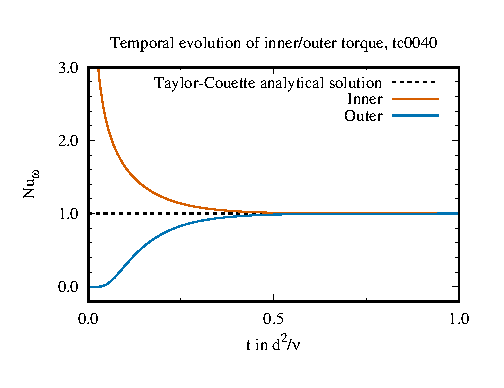
\includegraphics[scale=1.0, trim=0mm 0mm 0mm 6mm, clip=true]{figures/tc0040/torque}
\caption{Temporal evolution of the torque at the inner and outer cylinder
wall in our first Taylor-Couette tutorial \code{tc0040} with $\Rei=\num{50}$.
The torque is expressed in a non-dimensional way using a type of a Nusselt
number, which relates the actual torque to the torque of the laminar
Taylor-Couette analytical solution.}
\label{fig:tc0040torque}
\end{figure}
We see that the inner and outer torque values both monotonically converge to the 
theoretically predicted value of one after roughly $\orderof\left(1\right)$ 
viscous time units. This again makes total sense, since this is approximately 
the time span it should take for the presence of the driving inner wall to 
propagated to the opposing wall (at a distance $d=1$) solely by the action of 
viscosity. % and take effect everywhere in the flow domain.
\par Next, we take a 
look at the time series output of the velocity vector at some particular probe 
locations in the flow field, which will give us more local insights into the 
flow, where the torque provided us with rather global informations. By simply 
typing
\begin{lstlisting}[language=bash]
feldmann@darkstar:~/nsCouette/tc0040$ gnuplot probes.gpl
feldmann@darkstar:~/nsCouette/tc0040$ okular probes.pdf &
\end{lstlisting}
we generate a plot as shown in figure \ref{fig:tc0040probes}.
\begin{figure}[htb]
\centering
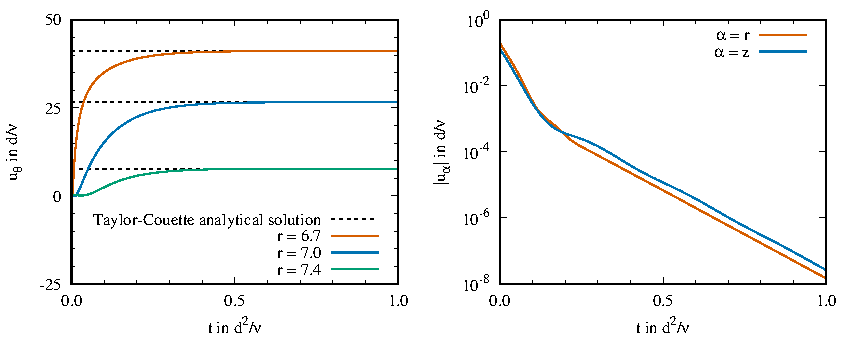
\includegraphics[scale=1.00]{figures/tc0040/probes}
\caption{Temporal evolution of the velocity components at individual probe 
locations in our first Taylor-Couette tutorial \code{tc0040} with $\Rei=\num{50}$.
The streamwise velocity component ($u_{\theta}$) is shown 
at three different radial locations ($r_{i}\le r\le r_{o}$) and converges 
everywhere to the theoretically predicted values (left). The absolute value of
the two cross-stream components ($|u_r|$ and $|u_z|$) is shown exemplarily at
one radial location ($r=\num{7.0}$).}
\label{fig:tc0040probes}
\end{figure}
We can easily see that the streamwise (azimuthal) velocity component 
($u_{\theta}$) converges nicely to the theoretically predicted values everywhere 
in the flow domain ($r_{i}\le r\le r_{o}$). As expected, both cross-stream 
velocity components ($|u_r|$ and $|u_z|$) decay to zero. The initial finite 
amplitude perturbations which we imposed do not survive in the linearly sable 
regime and the analytical solution for laminar Taylor-Couette flow is nicely 
reproduced/recovered. Information about the analytical Taylor-Couette solution can be 
found in the \code{probes.gpl} file by typing e.g.
\begin{lstlisting}[language=Gnuplot]
sed -n '18, 33 p' probes.gpl 

# Taylor-Couette set-up
Re_i = 50.0 # inner cylinder Reynolds number
Re_o =  0.0 # outer cylinder Reynolds number
eta = 0.868 # raddii ratio

# Analyitcal Taylor-Couette solution
nutc = 1.0 # Taylor-Couette analytical torque (Nusselt number)
c1 = (Re_o - eta * Re_i) / (1 + eta)
c2 = (eta * (Re_i - eta*Re_o)) / ((1 - eta) * (1 - eta**2.0))
r1 = 6.741192272578147 # radial probe location from file header
r2 = 7.023493344123748 # radial probe location from file header
r3 = 7.410322878937004 # radial probe location from file header
utc1 = c1*r1 + c2/r1  # Taylor-Couette analytical velocity
utc2 = c1*r2 + c2/r2  # Taylor-Couette analytical velocity
utc3 = c1*r3 + c2/r3  # Taylor-Couette analytical velocity
\end{lstlisting}
or e.g. in \cite{Shi2015} on page \num{5} and in \cite{Brauckmann2016} around 
page \num{424}. The particular radial probe locations for which the analytical 
solution is needed to produce figure \ref{fig:tc0040probes}, can be found in the 
header of the \code{probe0*.dat} files by typing
\begin{lstlisting}[language=bash]
feldmann@darkstar:~/nsCouette/tc0040$ head -n 10 probe01.dat
# Time series data from probe 01 on rank 00000
# Radial location n_r = 00005 n_rp = 0005 r =  6.741192272578147E+00
# Azimuthal location n_th = 00003 th =  2.617993877991494E-01
# Axial location n_z = 00003 z =  6.000000000000010E-01
# Time, u_r, u_th, u_z 
9.9900000000000E-004  4.9755347543047E-002 -5.0697872196875E-001  -3.9262289916098E-001
2.1090000000000E-003  4.9251475018859E-002  2.0445331579843E-003  -3.7513595580142E-001
3.2190000000000E-003  4.8415330734597E-002  1.4934842744334E+000  -3.5808738661681E-001
4.3290000000000E-003  4.7373835221887E-002  3.3163726265500E+000  -3.4181516483879E-001
5.4390000000000E-003  4.6167965547437E-002  5.1781059897116E+000  -3.2637614051804E-001
\end{lstlisting}
In case you are interested in time series data at different probe locations, you 
can modify the coordinates and the sampling rate in the parameter file using 
your favourite text editor
\begin{lstlisting}[language=Fortran]
feldmann@darkstar:~/nsCouette/tc0040$ vi nsCouette.in
&parameters_output
dn_prbs   = 10  ! output interval [steps] for time series data at probe locations
prl_r(1)  = 0.20d0 ! radial probe locations (0 < r/d < 1)
prl_r(2)  = 0.50d0
prl_r(3)  = 0.80d0
prl_r(4)  = 0.20d0
prl_r(5)  = 0.50d0
prl_r(6)  = 0.80d0
prl_th(1) = 0.25d0 ! azimuthal probe locations (0 < th/L_th < 1)
prl_th(2) = 0.25d0
prl_th(3) = 0.25d0
prl_th(4) = 0.75d0
prl_th(5) = 0.75d0
prl_th(6) = 0.75d0
prl_z(1)  = 0.25d0 ! axial probe locations (0 < z/L_z < 1)
prl_z(2)  = 0.25d0
prl_z(3)  = 0.25d0
prl_z(4)  = 0.75d0
prl_z(5)  = 0.75d0
prl_z(6)  = 0.75d0
/
\end{lstlisting}
and restart (Section~\ref{sec:checkpoint}) or rerun the simulation.
\par
Since we have only looked at particular points in the flow field so far,
figure \ref{fig:tc0040laminarTaylorCouette} shows a three-dimensional
view on the entire computational domain ($(r_{i}\le r\le r_{o}) \times
(\num{0}\le\theta\le L_{\theta}) \times (\num{0}\le z\le L_{z})$) we have
chosen for our first test case.
\begin{figure}[htb]
\centering
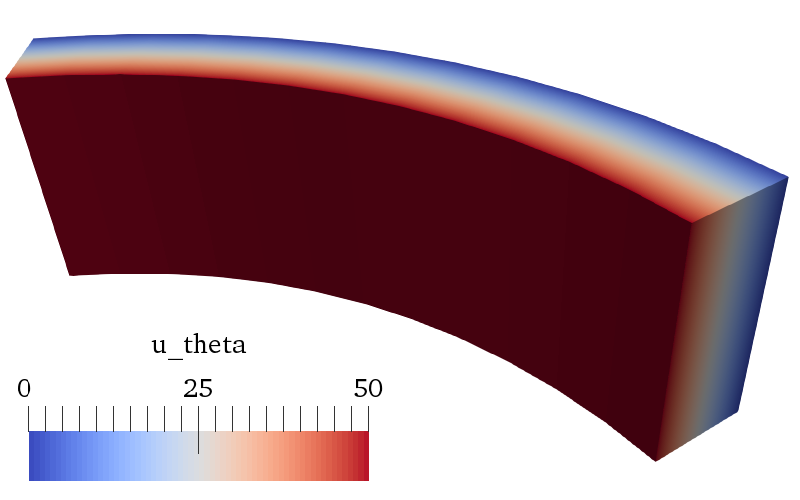
\includegraphics[width=1.00\textwidth]{figures/tc0040/laminarTaylorCouette.png}
\caption{The depicted volume represents the entire computational domain
($(\num{6.576}\le r\le\num{7.576}) \times (\num{0}\le\theta\le\sfrac{2\pi}{6})
\times (\num{0}\le z\le\num{2.4})$) we have chosen for our first DNS; i.e. only
one sixth of a full cylinder with a very small axial height. The colour-coding
represents the only non-zero velocity component ($u_{\theta}$), which is
obviously invariant with respect to $\theta$ and $z$ and only varies with
respect to the wall-normal location $r$ according to the analytical solution
for laminar Taylor-Couette flow.}
\label{fig:tc0040laminarTaylorCouette}
\end{figure}
To keep the simulation simple and quick, we restrict ourselves to only a segment of
a full real-world Taylor-Couette cylinder set-up. Here we chose one sixth of the
full azimuth ($L_{\theta}=\sfrac{2\pi}{k_{\theta,0}}=\sfrac{2\pi}{6}$) and only a
very small height of ($L_{z}=\sfrac{2\pi}{k_{z,0}}=\sfrac{2\pi}{2.618}=\num{2.4}$),
as can be specified by setting
\begin{lstlisting}[language=Fortran]
&parameters_grid
k_th0 = 6.0d0               ! azimuthal fundamental wavenumber
k_z0  = 2.61799387799149d0  ! axial fundamental wavenumber
eta   = 0.868d0             ! inner to outer radii aspect ratio
\
\end{lstlisting}
in the namelist \code{parameters\_grid} in the parameter input file.
The colour-coding in figure \ref{fig:tc0040laminarTaylorCouette} represents
the only non-zero velocity component
\begin{align}
\vec{u}=
\begin{bmatrix}
u_{r}\\ u_{\theta}\\u_{z}
\end{bmatrix}
=
\begin{bmatrix}
0\\ f(r)\\0
\end{bmatrix}
\text{,} 
\end{align}
which is obviously invariant with respect to the azimuth $\theta$ and the axial
location $z$. It only varies with respect to the wall-normal location $r$ and
decreases monotonically from the inner cylinder wall at $r=r_{i}=\num{6.576}$,
which is driven at a speed of $\num{50}\sfrac{d}{\nu}$, down to zero at the outer
cylinder wall ($r=r_{o}=\num{7.576}$), which is kept stationary. This pseudo-colour
representation of the flow field can be easily reproduced using \code{ParaView}
and loading the state file \code{la\-mi\-nar\-Tay\-lor\-Cou\-ette.pvsm} which comes with this
tutorial. Further details on how to visualise flow fields can be found in
section~\ref{sec:paraview} or section~\ref{sec:visit}, in case you prefer the software
\code{VisIt}.
\par
Last but not least we want to have a look at the time series data for the
kinetic energy. The two files \code{ke\_th} and \code{ke\_z} provide integral
kinetic energies for each discrete Fourier mode ($n_{\theta}$ and $l_{z}$,
respectively) at each time step. So in our case, both files contain six
columns of time series data: the  first one being the physical time $t$ and
the next five being the integral kinetic energy in mode number
$\num{0}\le n_{\theta}\le N=\num{4}$ and $\num{0}\le l_{z}\le L=\num{4}$,
respectively. The kinetic energy per mode is an integral quantity in the sense,
that it is integrated in both cases over the radial direction ($r$) and also
over either the axial ($z$) or the azimuthal ($\theta$) direction, respectively,
depending on which quantity you are looking at.
By simply typing
\begin{lstlisting}[language=bash]
feldmann@darkstar:~/nsCouette/tc0040$ gnuplot keThZ.gpl
feldmann@darkstar:~/nsCouette/tc0040$ okular keThZ.pdf &
\end{lstlisting}
we generate a plot as shown in figure~\ref{fig:tc0040keThZ}.
\begin{figure}[htb]
\centering
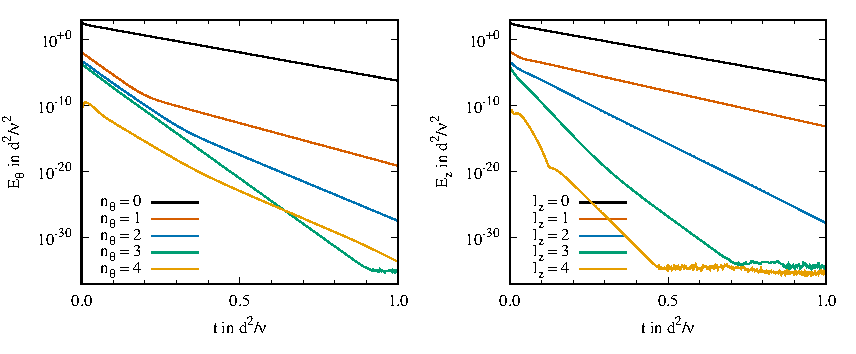
\includegraphics[scale=1.00]{figures/tc0040/keThZ.pdf}
\caption{Temporal evolution of the azimuthally (left) and axially (right) 
dependent kinetic energy contained in each discrete azimuthal ($n_{\theta}$)
and axial ($l_{z}$) mode for our first Taylor-Couette tutorial \code{tc0040}
with $\Rei=\num{50}$. See also page 3 in \cite{Shi2015} for definitions and 
details on the spatial discretisation scheme of \nsc. As expected, the non-zero 
kinetic energy introduced by the finite amplitude perturbation in the initial 
velocity field decays monotonically to practically zero in all modes and never 
increases again.}
\label{fig:tc0040keThZ}
\end{figure}
Since there is no relevant energy content in any of the modes larger than the zero 
mode (which represents the mean value in the respective direction), there is no
variation of the flow field neither in $\theta$ nor in $z$ direction. And there is
obviously also no periodic or chaotic variation with respect to time at this low
Reynolds number. Actually, the kinetic energy in all modes decays to practically
zero. The amount of energy introduced to the initial conditions by the finite amplitude
perturbations is monotonically damped out by the dominating effect of viscosity and it
never increases again. You can easily double-check this for larger times by simply
restarting (Section \ref{sec:checkpoint}) the simulation and let it run for another
\num{8000} or more time steps. Although the dynamics at this low Reynolds number is
rather boring and also trivial as well as expected, these per mode energies are a
very convenient and important measure to track and analyse the dynamical behaviour
of the Taylor-Couette system in general. However, have in mind, that for more
interesting (i.e. increasing) Reynolds numbers -- and thus finer spatial resolution -- these
files progressively become huge and are not so easy to handle anymore. One option
could be to increase the sampling frequency for these specific output. This can be done
using the respective keyword in the namelist \code{parameters\_output} in the parameter input file.
\begin{lstlisting}[language=fortran]
feldmann@darkstar:~/nsCouette/tc0040$ vi nsCouette.in  
&parameters_output
dn_ke = 1000   ! Time step output interval for modal kinetic energy
/
\end{lstlisting}
Additionally, the highest wave numbers represent the spatial resolution of the
simulation. Here, they only show numerical noise nut no relevant energy content.
Plots like these in figures~\ref{fig:tc0040keThZ}, \ref{fig:tc0040keThZ} and
\ref{fig:tc0040keThZ}
become very handy as an indicator
for the quality of the spatial resolution. Although the details very much depend on
what exactly you are intending to do, as a rough rule the energy should decay
at least several (five, six, seven \dots) orders of magnitude from the lowest to the
highest wave number (at all times in the simulation) to consider the spatial resolution
as sufficient. 


\subsection{Taylor-vortex flow}
\label{sec:tc0041}

Above a certain Reynolds number -- slightly depending on the exact geometry and
boundary conditions -- the Taylor-Couette flow becomes unstable and gives rise
to Taylor vortices. In a next step, we want to increase the Reynolds number to
the unstable regime and see whether \nsc reproduces this well known Taylor-vortex
state. Go back to your working directory, copy the second Taylor-Couette tutorial
case from the repository and inspect the parameter file (\code{nsCouette.in})
using your favourite text editor.
\begin{lstlisting}[language=bash]
feldmann@darkstar:~$ cd ~/nsCouette
feldmann@darkstar:~/nsCouette$ cp -r ../nscouette/tutorials/tc0041 .
feldmann@darkstar:~/nsCouette$ cd tc0041
feldmann@darkstar:~/nsCouette/tc0041$ vi nsCouette.in
\end{lstlisting}
We triple the rotation speed of the inner cylinder by changing the respective
keywords in the namelist \code{parameters\_physics}. Since we now expect a slightly
more complex flow field, we also have to increase the spatial resolution to
account for the spatial velocity gradients related to the pronounced vortex
in the flow field.
\begin{lstlisting}[language=Fortran]
&parameters_physics
Re_i = 150.0d0 ! inner cylinder Reynolds number
Re_o =   0.0d0 ! outer cylinder Reynolds number
/
&parameters_grid
m_r  = 24   ! M radial points
m_th =  4   ! N azimuthal Fourier modes
m_z0 =  8   ! L axial Fourier modes
/
\end{lstlisting}
This choice corresponds to a total of $n_r \times n_\theta  \times n_z=M \times
(2N+1) \times (2L+1) = \num{24} \times \num{9} \times \num{17}$ significant
physical grid points. The finer spatial resolution naturally demands a smaller
computational time step $\Delta t$. Since $\Delta t$ will be adapted automatically
to ensure numerical stability during integration, we simply have to increase the
total number of time steps in namelist \code{parameters\_timestep}, to end up at
roughly the same physical time $t$ as in our first tutorial case
(Section~\ref{sec:tc0040}).
\begin{lstlisting}[language=Fortran]
&parameters_timestep
numsteps    = 22000   ! Number of computational time steps
variable_dt = T       ! Use variable (T) or fixed (F) time step size
/
\end{lstlisting}
Both changes will
surely increase the overall computational time necessary for our second DNS.
To save resources and to keep the tutorials small, we now choose start our
second simulation from a flow state similar to the one we ended up with in our
first tutorial (Section~\ref{sec:tc0040}). We do this by prescribing the analytical
Taylor-Couette velocity profile as initial condition and again add a finite
amplitude perturbation on top of it.
\begin{lstlisting}[language=Fortran]
feldmann@darkstar:~/nsCouette/tc0041$ vi nsCouette.in
&parameters_initialcondition
ic_tcbf = T ! Set Taylor-Couette base flow (T) or resting fluid (F), only when restart = 0
ic_pert = T ! Add perturbation on top of base flow (T) or not (F), only when restart = 0
ic_p(1, :) = 4.0d-2, 0, 1 ! 1st perturbation: amplitude and wavevector (a1, k_th1, k_z1)
ic_p(2, :) = 6.0d-3, 1, 0 ! 2nd perturbation: amplitude and wavevector (a2, k_th2, k_z2)
/
\end{lstlisting}
To run this tutorial, you now simply have to copy the same executable as before
(Section~\ref{sec:tc0040}) to the new case directory and start the simulation by
prompting the executable and passing the new parameter input file to the standard input.
Further details and different ways to start a simulation can be found in
section~\ref{sec:runningTheCode}. 
\begin{lstlisting}[language=bash]
feldmann@darkstar:~/nsCouette/tc0041$ cp ../nscouette/darkstar/nsCouette.x .
feldmann@darkstar:~/nsCouette/tc0041$ ./nsCouette.x < nsCouette.in
...
  step=       19000  dt=   6.6666666666666670E-005
  step=       20000  dt=   6.6666666666666670E-005
  step=       21000  dt=   6.6666666666666670E-005
 written hdf5/xdmf files to disk: fields_tc0041_00022000.{h5,xmf}
  step=       22000  dt=   6.6666666666666670E-005
 written coeff file to disk: coeff_tc0041.00022000                   
 written coeff file to disk: coeff_tc0041.00022000                   
------------------------------------------------------------------------------------
Total number of timesteps: 00022000
Total elapsed WCT:    26.96s
Elapsed WCT per time step w/o coeff io (min, max, average):   0.0012s,    0.0012s,    0.0012s
\end{lstlisting}
Now \nsc runs on one single \mpi task and throws its log output directly
to the terminal. You can watch the progress of the simulation step by step,
which should usually finish in less than a minute (Here after \SI{26.96}{\second}).
\par
Let's continue with first having a look at the final flow state.
Figure~\ref{fig:tc0041vectorPlot} shows a three-dimensional representation
of the instantaneous flow field at the last time step from our simulation run.
\begin{figure}
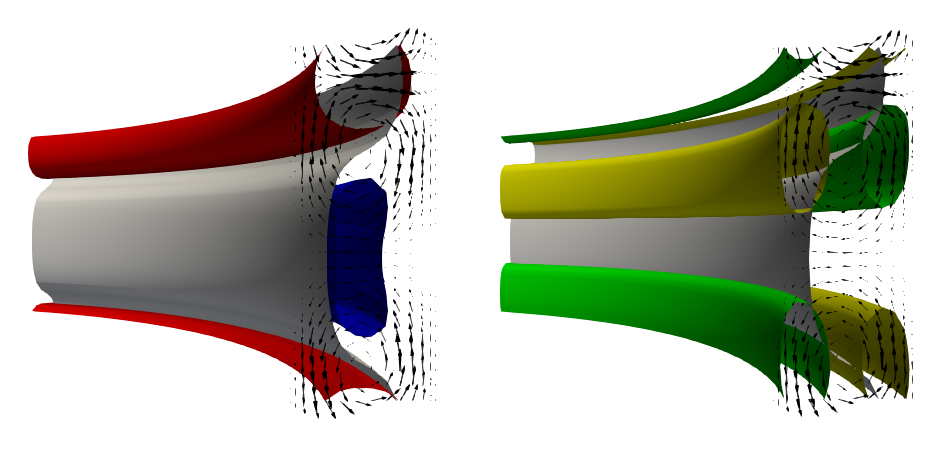
\includegraphics[width=1.00\textwidth]{figures/tc0041/vectorPlot.png}
\caption{Three-dimensional flow field visualisation using \code{ParaView}.
Shown are iso-contours (red/blue: $u_{r}=\pm\num{4}$, grey:
$u_{\theta}=\num{75}$, yellow/green: $u_{z}=\pm\num{4}$) and a vector
representation of the cross-stream velocity components. Stationary
Taylor-vortex flow state at $\Rei=\num{150}$.}
\label{fig:tc0041vectorPlot}
\end{figure}
As already mentioned above, the higher Reynolds number now gives rise
to a spatially more complex state with a secondary flow ($u_{r,z}\neq\num{0}$)
forming toroidal vortices. As shown in figure~\ref{fig:tc0041vectorPlot},
alternating regions of positive (red) and negative (blue) $u_r$ push high-speed
fluid from the rotating inner cylinder towards the stationary outer cylinder;
And Vice versa for low-speed fluid. This can be easily seen by the bent
iso-surface (grey) representing the average streamwise velocity 
($u_{\theta}=\sfrac{\left(\Rei+\Reo\right)}{2}$) between the cylinders.
To fulfil mass conservation, these regions are flanked by four alternating regions of
axial up (green) and down (yellow) wash. This well-known phenomenon is a so-called
Taylor-Vortex (TV), which is more thoroughly discernible through the vector representation
of the two cross-stream velocity components $u_{r}$ and $u_{z}$, which are also included
in figure~\ref{fig:tc0041vectorPlot}. You can easily create such plot with \code{ParaView}
by loading the corresponding \code{*.h5} file (Section \ref{sec:}), performing a coordinate
transformation (Section \ref{sec:}) and playing around with the \code{contour},
\code{slice} and \code{glyph} filters. Loading the provided state file (\code{taylorVortexIsoContourVectorPlot.pvsm}) might also be helpful to learn creating such plots.
\par
The Taylor-Vortex state -- which is reached after a certain transient phase -- is
invariant in $\theta$ (axisymmetric) and also invariant in $t$ (stationary). The
first one can be easily seen from the discussed flow field representation shown
in figure~\ref{fig:tc0041vectorPlot}. The latter one can be easily seen from the
time series of $u_{\theta}$ shown in figure~\ref{fig:tc0041probes}.
\begin{figure}[htb]
\centering
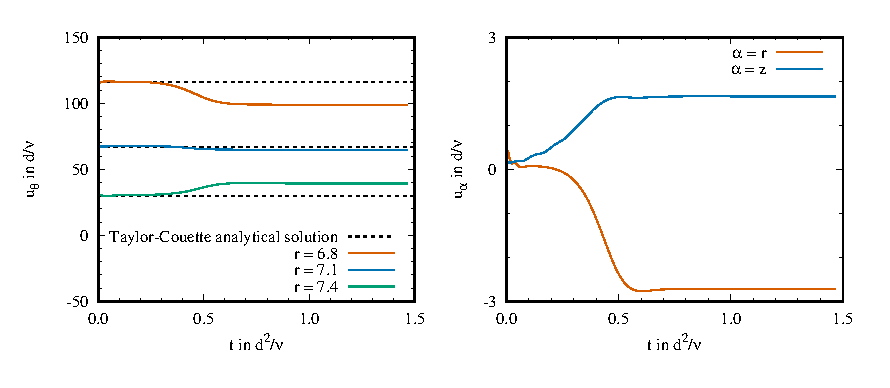
\includegraphics[scale=1.00]{figures/tc0041/probes}
\caption{Temporal evolution of the velocity components at individual probe 
locations in our second Taylor-Couette tutorial \code{tc0041} with $\Rei=\num{150}$.
The streamwise velocity component ($u_{\theta}$) is shown 
at three different radial locations ($r_{i}\le r\le r_{o}$) and converges 
everywhere to a constant value different from the theoretically predicted values for
the simple Taylor-Couette flow state. The values of the two cross-stream components
($u_r$ and $u_z$) also converges to constant but non-zero value, as shown exemplarily
at one radial location ($r=\num{7.0}$).}
\label{fig:tc0041probes}
\end{figure}
The streamwise velocity component recorded at three different radial
locations ($r_{i}\le r\le r_{o}$) converges everywhere to a constant
value, which is, however, different from the one theoretically predicted
for the simpler Taylor-Couette flow state. Note, that this time we
started our simulation from the analytical Taylor-Couette flow field
and not from a resting fluid


The values of the two
cross-stream components ($u_r$ and $u_z$) also converge to constant
but non-zero values after a certain transient phase. Due to the presence
of a Taylor-Vortex pair, stronger velocity gradients occur near the
walls. These stronger gradients lead to higher shear-stresses and thus
to higher torque values compared to pure Taylor-Couette flow state,
as can be seen in figure~\ref{fig:tc0041torque}.
\begin{figure}[htb]
\centering
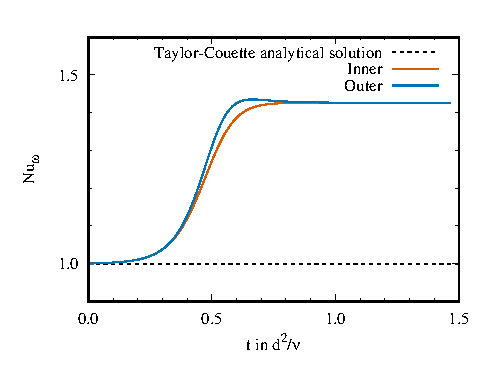
\includegraphics[scale=1.0, trim=0mm 0mm 0mm 0mm, clip=true]{figures/tc0041/torque}
\caption{Temporal evolution of the torque at the inner and outer cylinder
wall in our second Taylor-Couette tutorial \code{tc0041} with $\Rei=\num{150}$.
The torque is expressed in a non-dimensional way using a type of a Nusselt
number, which relates the actual torque to the torque of the laminar
Taylor-Couette analytical solution.}
\label{fig:tc0041torque}
\end{figure}

\begin{figure}[htb]
\centering
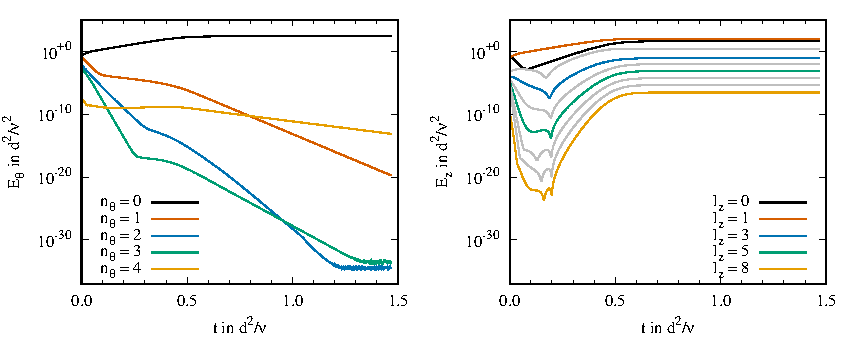
\includegraphics[scale=1.00]{figures/tc0041/keThZ.pdf}
\caption{Temporal evolution of the azimuthally (left) and axially (right) 
dependent kinetic energy contained in each discrete azimuthal ($n_{\theta}$)
and axial ($l_{z}$) mode for our second Taylor-Couette tutorial \code{tc0041}
with $\Rei=\num{150}$.}
\label{fig:tc0041keThZ}
\end{figure}


The plots shown in figures~\ref{fig:tc0041probes}, \ref{fig:tc0041torque},
\ref{fig:tc0041keThZ} can be easily reproduced with the ready-to-use
\code{gnuplot} scripts provided in this tutorial.
\begin{lstlisting}[language=bash]
feldmann@darkstar:~/nsCouette/tc0041$ gnuplot probes.gpl
feldmann@darkstar:~/nsCouette/tc0041$ gnuplot torque.gpl
feldmann@darkstar:~/nsCouette/tc0041$ gnuplot keThZ.gpl
feldmann@darkstar:~/nsCouette/tc0041$ okular probes.pdf torque.pdf keThZ.pdf &
\end{lstlisting}




% \begin{lstlisting}[language=bash]

% \end{lstlisting}


% \begin{lstlisting}[language=bash]
% feldmann@darkstar:~$ cd nsCouette/tc0041
% feldmann@darkstar:~/nsCouette/tc0041$ cp ../nscouette/darkstar/nsCouette.x .
% feldmann@darkstar:~/nsCouette/tc0041$ ./nsCouette.x < nsCouette.in
% \end{lstlisting}




\subsection{Wavy vortex flow}
\label{sec:tc0042}

Figrues \ref{fig:tc0042torque} to \ref{fig:tc0042keThZ} show the results for
a wavy vortex flow state simulation, which can be reproduced analogue to the
detailed description in tutorial \ref{sec:tc0040} and \ref{sec:tc0041}. More
tutorials will follow in the future!



\begin{figure}[htb]
\centering
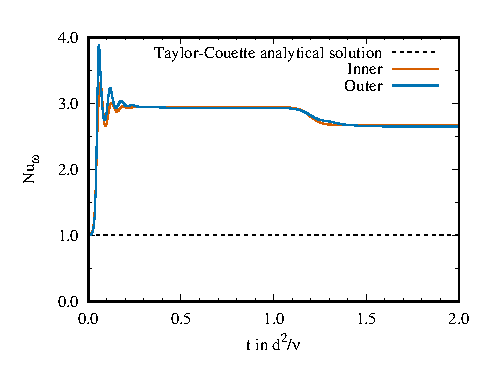
\includegraphics[scale=1.0]{figures/tc0042/torque}
\caption{Temporal evolution of the torque at the inner and outer cylinder
wall in our third Taylor-Couette tutorial \code{tc0042} with $\Rei=\num{458.1}$.
The torque is expressed in a non-dimensional way using a type of a Nusselt
number, which relates the actual torque to the torque of the laminar
Taylor-Couette analytical solution.}
\label{fig:tc0042torque}
\end{figure}

\begin{figure}[htb]
\centering
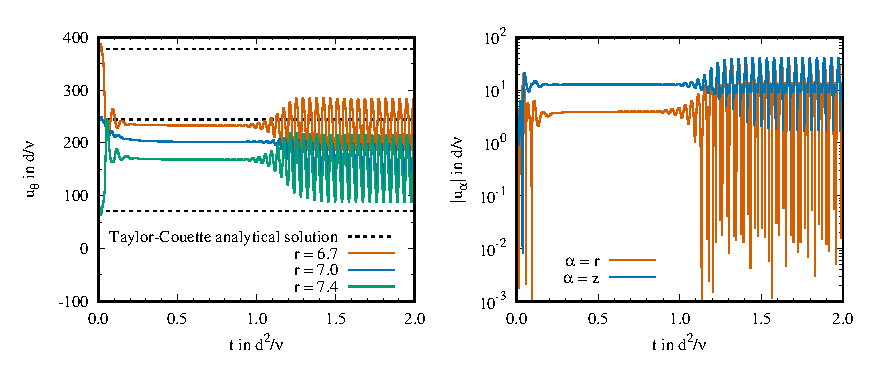
\includegraphics[scale=1.00]{figures/tc0042/probes}
\caption{Temporal evolution of the velocity components at individual probe 
locations in our third Taylor-Couette tutorial \code{tc0042} with $\Rei=\num{458.1}$.
The streamwise velocity component ($u_{\theta}$) is shown 
at three different radial locations ($r_{i}\le r\le r_{o}$) and converges 
everywhere to the theoretically predicted values (left). The absolute value of
the two cross-stream components ($|u_r|$ and $|u_z|$) is shown exemplarily at
one radial location ($r=\num{7.0}$).}
\label{fig:tc0042probes}
\end{figure}

\begin{figure}[htb]
\centering
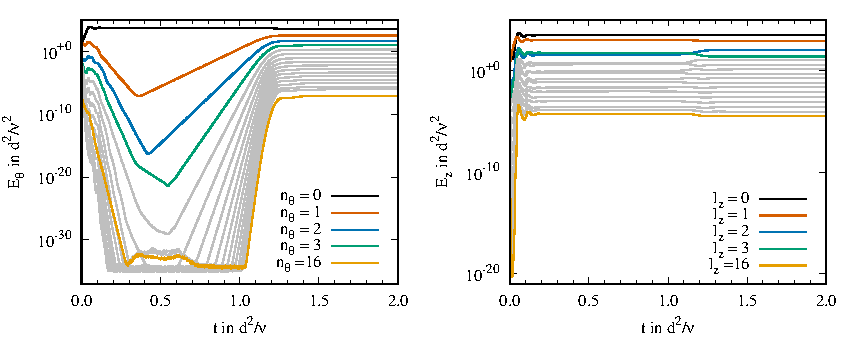
\includegraphics[scale=1.00]{figures/tc0042/keThZ.pdf}
\caption{Temporal evolution of the azimuthally (left) and axially (right) 
dependent kinetic energy contained in each discrete azimuthal ($n_{\theta}$)
and axial ($l_{z}$) mode for our third Taylor-Couette tutorial \code{tc0042}
with $\Rei=\num{458.1}$. See also page 3 in \cite{Shi2015} for definitions and 
details on the spatial discretisation scheme of \nsc. As expected, the non-zero 
kinetic energy introduced by the finite amplitude perturbation in the initial 
velocity field decays monotonically to practically zero in all modes and never 
increases again.}
\label{fig:tc0042keThZ}
\end{figure}



\subsection{Thermal convection}
\label{sec:tc0073}

The flow of air between a hot rotating cylinder and a cooled stationary
cylindrical enclosure is a simple model to investigate heat transfer in
rotating machines~\cite{Howey2012}. At low rotation rates and small temperature differences,
the heat transfer is purely conductive and the flow has only an azimuthal
component. In this simple case, the governing equations admit a simple
analytic solution, termed basic state, whose temperature and velocity
profiles depend only on the radial coordinate, see e.g. equations (2) to (4)
in \cite{Lopez2015}. Heat transfer can be enhanced by either increasing the
speed of the inner cylinder (forced convection), or by increasing the
temperature difference (natural convection). In both cases, the basic state exhibits
a sequence of distinct instabilities leading to turbulent heat transfer~\cite{Lopez2015}. A
measure of the efficiency is given by the Nusselt number \Nui, which is the
ratio of total heat transfer at the inner cylinder, normalised by the heat transfer
of the purely conductive basic state at the same temperature difference.
\par
Here, we want to reproduce this behaviour in a series of three short DNS runs.
First, you have to build the temperature version (\code{TE\_CODE}) of \nsc,
as described in section~\ref{sec:buildingTheCode}.
Once this is done, go to your working directory, copy the first thermal convection
tutorial case from the repository
\begin{lstlisting}[language=bash]
cd ~/nsCouette
cp -r ../nscouette/tutorials/tc0073 .
cd tc0073
vi nsCouette.in
\end{lstlisting}
and inspect the parameter file (\code{nsCouette.in}) using your favourite 
text editor.



In this tutorial case directory you can find two ready-to-use scripts to
generate the time series plots shown in figure \ref{fig:compareGrass} by
simply typing
\begin{lstlisting}[language=bash]
gnuplot probeCompare.gpl
gnuplot torqueCompare.gpl
okular probeComapre torqueCompare.pdf &
\end{lstlisting}
and opening the generated \code{*.pdf} figures using your favourite document 
viewer (e.g. \code{okular}, \code{evince}, \code{acroread} and alike).


Now we want to increase the effect of thermal convection by increasing the
temperature difference between the inner and outer cylinder wall. In \nsc
this can be done by specifying a larger Grashof number. Got back to your working
directory, copy the next convection tutorial case and inspect the input file
\begin{lstlisting}[language=bash]
cd ~/nsCouette
cp -r ../nscouette/tutorials/tc0075 .
cd tc0075
vi nsCouette.in
\end{lstlisting}
using your favourite text editor. Note, that we now have increased \Gr to \num{4000}
and that we have also increased the axial resolution, since we expect a slightly more
complex flow state. Moreover, we now want to run the simulation for another
\num{400000} time steps (instead of \num{200000} as before) to end up with roughly
the same physical time span, since we now expect a slightly smaller $\Delta t$ due to
larger velocities and a finer grid resolution:
\begin{lstlisting}[language=fortran]
vi nsCouette.in
&parameters_grid
...
m_z0 = 32  ! L axial Fourier modes => 2*m_z0+1 grid points (axial)
/
&parameters_physics
...
Gr = 4000.0d0 ! Grashof number Gr = Ra/Pr [TE_CODE only]
/
&parameters_timestep
...
numsteps = 400000   ! number of computational time steps
/
&parameters_output
...
fBase_ic = 'tc0075' ! identifier for coeff_ (checkpoint) and fields_ (hdf5) files
/
&parameters_control
...
restart = 1   ! initial conditions, start from: 0=scratch, 1,2=checkpoint
/  
\end{lstlisting}


To specify the initial conditions, create a symbolic link to the last flow field snapshot
from the former DNS at the lower \Gr
\begin{lstlisting}[language=bash]
ln -s ../tc0073/coeff_tc0073.00200000 coeff_tc0075.00200000
cp ../tc0073/coeff_tc0073.00200000.info restart
\end{lstlisting}
and also create a file \code{restart} from the corresponding \code{*.info} file.
The file \code{restart} has to be slightly modified to account for the new case/base
name
\begin{lstlisting}[language=bash]
vi restart
&parameters_restart
...
fbase_ic = tc0075
/
&parameters_info
...
/
\end{lstlisting}
using your favourite text editor.


\begin{figure}[htb]
\centering
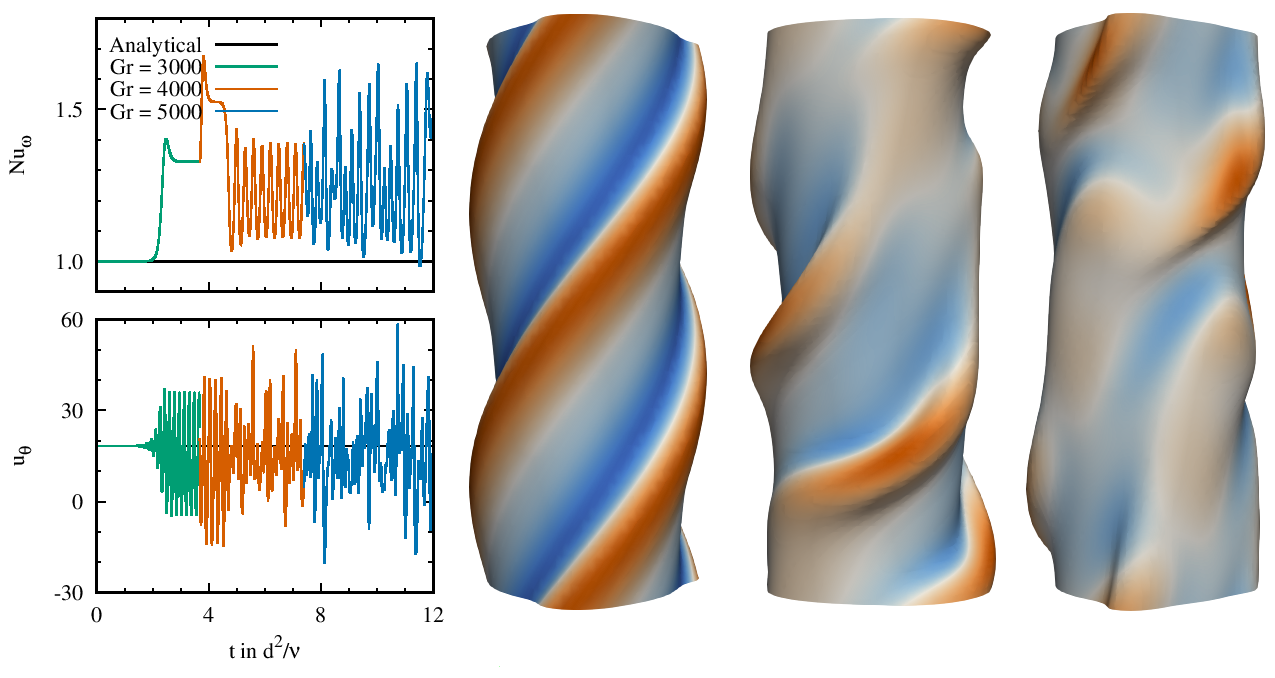
\includegraphics[width=1.00\textwidth]{figures/tc0073/compareGrasshof.png}
\caption{Different flow states for increasing Grass number when restarted
the simulation from a former run. Temporal evolution of the torque at the inner
cylinder wall and the streamwise (azimuthal) velocity component at one mid-gap
probe location. Iso-surfaces of the mean Temperature ($T=0$) colour-coded by the
inwards (blue) and outwards (r) directed wall-normal (radial) velocity component.}
\label{fig:compareGrass}
\end{figure}





\appendix



\section{List of parameters}
\label{sec:listOfParameters}

Starting with \nsc version \code{1.0}, the file \code{mod\_params.f90} needs
no more editing before building the code. Instead, most of the settings and
parameters can be specified at run-time as described in section~\ref{sec:parameterInputFile}.
So in general, \nsc has to be build only once on a system. The same executable
can be used for all your simulations within one project, as long as you don't
want to change something in the code or want to switch to e.g. simulations with
thermal convection. The latter one is described in section~\ref{sec:thermalConvection}
and in the tutorials section~\ref{sec:tc0073}. Another example for when you need to
modify source files and rebuild the code, is changing the parameters of the time
stepper, which is detailed in section~\ref{sec:timeStepper}.
\par
For reference and completeness, we here print the \code{mod\_params.f90} file
from a pre-\code{1.0} code version; also in order to document the geometrical
and numerical parameters that were used for the example of Figure 5 in our CAF
paper~\cite{Shi2015}. The variable names in the source code are more or less
compatible with the symbols and notation used in our CAF paper.
\begin{lstlisting}[language=Fortran]
INTEGER(KIND=4),PRIVATE   :: ir
!--- Mathematical constants
REAL(KIND=8)   ,PARAMETER :: epsilon = 1D-10  ! numbers below it = 0
REAL(KIND=8)   ,PARAMETER :: PI = ACOS(-1d0)  ! pi = 3.1415926...
COMPLEX(KIND=8),PARAMETER :: ii = DCMPLX(0,1) ! Complex i = sqrt(-1)

!--- Spectral parameters
INTEGER(KIND=4),PARAMETER :: m_r  = 32  ! Maximum spectral mode (> n_s-1)
INTEGER(KIND=4),PARAMETER :: m_th = 16  ! Number of Fourier modes
INTEGER(KIND=4),PARAMETER :: m_z0 = 16 
INTEGER(KIND=4),PARAMETER :: m_z = 2*m_z0 
INTEGER(KIND=4),PARAMETER :: m_f  = (m_th+1)*m_z ! Total number of Fourier modes
REAL(KIND=8)   ,PARAMETER :: k_th0= 6.D0   ! Minimum azimuthal wavenumber
REAL(KIND=8)   ,PARAMETER :: k_z0 = 2*PI/2.4  ! Minimum axial wavenumber

!--- Physical parameters
INTEGER(KIND=4),PARAMETER :: n_r  = m_r ! Number of grid points
INTEGER(KIND=4),PARAMETER :: n_th = 2*m_th
INTEGER(KIND=4),PARAMETER :: n_z  = m_z
INTEGER(KIND=4),PARAMETER :: n_f  = n_th*n_z  ! Number of points in Fourier directions
REAL(KIND=8)   ,PARAMETER :: len_r  = 1d0  ! Physical domain size
REAL(KIND=8)   ,PARAMETER :: len_th = 2*PI/k_th0
REAL(KIND=8)   ,PARAMETER :: len_z  = 2*PI/k_z0
REAL(KIND=8)   ,PARAMETER :: eta = 8.68d-1 ! Radii ratio r_i/r_o
REAL(KIND=8)   ,PARAMETER :: r_i = eta/(1-eta)   ! Inner radius
REAL(KIND=8)   ,PARAMETER :: r_o = 1/(1-eta)  ! Outer radius
REAL(KIND=8)   ,PARAMETER :: r(n_r) = (/(((r_i+r_o)/2 &
- COS(PI*ir/(n_r-1))/2), ir=0,(n_r-1))/) ! Chebyshev distribution for radial points
REAL(KIND=8)   ,PARAMETER :: th(n_th) = (/(ir*len_th/n_th,ir=0,n_th-1)/)
REAL(KIND=8)   ,PARAMETER :: z(n_z) = (/(ir*len_z/n_z,ir=0,n_z-1)/)
REAL(KIND=8)   ,PARAMETER :: gap = 3.25d0  ! gap size in cm
REAL(KIND=8)   ,PARAMETER :: gra = 980  ! gravitational acceleration in g/cm**3
REAL(KIND=8)   ,PARAMETER :: nu = 1.01d-2  ! kinematic viscosity in cm**2 /s

!--- Time stepper
REAL(KIND=8), PARAMETER :: d_implicit = 0.51d0  ! implicitness
REAL(KIND=8), PARAMETER :: tolerance_dterr = 5.0d-5   ! tolerance for corrector step

!--- MPI & FFTW parameters
INTEGER(KIND=4), PARAMETER :: root = 0   ! Root processor
INTEGER(KIND=4), PARAMETER :: fftw_nthreads = 1
LOGICAL  , PARAMETER :: ifpad = .TRUE.   ! If apply '3/2' dealiasing

!--- Finite differences parameters
INTEGER(KIND=4),PARAMETER :: n_s = 9 ! Leading length of stencil

!--- Defaults for runtime parameters
REAL(KIND=8) :: Courant = 0.25d0
INTEGER(KIND=4) :: print_time_screen = 250
LOGICAL   :: variable_dt= .true.
REAL(kind=8) :: maxdt = 0.01d0
INTEGER(KIND=4) :: numsteps = 100000 ! Number of time steps
INTEGER(KIND=4) :: dn_coeff = 5000   ! Output coefficients every nth step
INTEGER(KIND=4) :: dn_ke = 100 ! Output energy every nth step
INTEGER(KIND=4) :: dn_vel = 100   ! Output velocity every nth step
INTEGER(KIND=4) :: dn_Nu = 100 ! Output Nusselt every nth step
INTEGER(KIND=4) :: dn_hdf5 = 1000 ! Output HDF5 every nth step
\end{lstlisting}



 
















\section{Configure and build additional software manually}
\label{app:selfBuildLibraries}

\subsection{Build \code{zlib}}
\label{sec:buildzlib}

This is a detailed description of how to manually build \code{zlib}
libraries on our local \code{fsmcluster} at the
\href{https://www.zarm.uni-bremen.de/en/}{ZARM} institute. This is required
for installing \hdf, as described in section~\ref{sec:buildhdf}

\begin{lstlisting}[language=bash]
# Brief comments on how to install zlib locally on fsmcluster@zamr, which is
# needed for HDF5, which is needed for NetCDF with netcdf-4 capabilities.
#
# Daniel Feldmann, 18th January 2017
# 
# Download and unpack to some directory of your choice, e.g. ~/zlib/build
tar xfvz zlib-1.2.11.tar.gz
cd zlib-1.2.11/
#
#
# Load Intel compiler suite available on fsmclsuter
module purge
module load Intel/PSXE2017
source /home/centos/Intel/PSXE2017/bin/ifortvars.sh intel64
source /home/centos/Intel/PSXE2017/bin/compilervars.sh intel64
source /home/centos/Intel/PSXE2017/bin/iccvars.sh intel64
#
# Check compiler version
module list
mpiicc --version
#
# Use Intel C compiler for the following steps, whatever icc or mpiicc, is not
# important as far as I know...
# export CC=icc
export CC=mpiicc
export CFLAGS="-O3 -xHost -ip -mcmodel=medium"
#
# Configure zlib to be installed into some place of you wish, e.g. as follows 
mkdir ~/zlib/zlib-1.2.11
./configure --prefix=/home/feldmann/zlib/zlib-1.2.11 
#
# Build, test and install zlib via
make
make check
make install
#
# Do not forget to unset environment varibles, which might mess up future builds
unset CC
unset CFLAGS
#
# You may need to add the path to the newly installed library to the
# LD_LIBRARY_PATH environment variable if that lib directory is not searched by
# default. E.g. put the following line to your ~/.bashrc
export LD_LIBRARY_PATH=$LD_LIBRARY_PATH:/home/feldmann/zlib/zlib-1.2.11/lib
# 
# Done!
\end{lstlisting}

This is a detailed description of how to manually build \code{zlib}
libraries on my local desktop machine, which might be useful as
a rough guide line. This is required
for installing \hdf, as described in section~\ref{sec:buildhdf}
\begin{lstlisting}[language=bash]
# Brief comments on how to install zlib locally on darkstar@zarm, which is
# needed for HDF5, which is needed for NetCDF with netcdf-4 capabilities.
#
# Daniel Feldmann, 6th January 2017
# 
tar xfvz zlib-1.2.11.tar.gz
cd zlib-1.2.11/
#
#
# Install openmpi and GNU C compiler if not already installed, both easily
# available via the package manager
sudo apt-get install openmpi-bin openmpi-common libopenmpi1.10 libopenmpi-dev mpi-default-bin mpi-default-dev
sudo apt-get install gcc gfortran g++
#
# Check compiler version
which mpicc
mpicc --version
#
# Use GNU C compiler for the following steps, whatever gcc or mpicc, is not
# important as far as I know...
# export CC=gcc
export CC=mpicc
export CFLAGS='-O3 -mcmodel=medium'
#
# Configure zlib to be installed into some place you wish, e.g. as follows 
mkdir ~/zlib/zlib-1.2.11
./configure --prefix=~/zlib/zlib-1.2.11
#
# Build, test and install zlib via
make
make check
make install
#
# Do not forget to unset environment varibles, which might mess up subsequent builds
unset CC
unset CFLAGS
#
# You may need to add the path to the newly installed library to the
# LD_LIBRARY_PATH environment variable if that lib directory is not searched by
# default. E.g. put the following line to your ~/.bashrc
export LD_LIBRARY_PATH=$LD_LIBRARY_PATH:/home/feldmann/zlib/zlib-1.2.11/lib
# 
# Done!
\end{lstlisting}



\subsection{Build \hdf}
\label{sec:buildhdf}
This is a detailed description of how to manually build \mpi-parallel \hdf
libraries with \fortran interfaces on our local \code{fsmcluster} at the
\href{https://www.zarm.uni-bremen.de/en/}{ZARM} institute. This requires
a \code{zlib} installation, as described in section~\ref{sec:buildzlib}

\begin{lstlisting}[language=bash]
# 
# Download and unpack to some directory of your choice, e.g. ~/hdf5/build/.
tar xvf hdf5-1.10.0-patch1.tar 
cd hdf5-1.10.0-patch1
#
# Load Intel compiler suite
module purge
module load Intel/PSXE2017
source /home/centos/Intel/PSXE2017/bin/ifortvars.sh intel64
source /home/centos/Intel/PSXE2017/bin/compilervars.sh intel64
source /home/centos/Intel/PSXE2017/bin/iccvars.sh intel64
#
# Check compiler version
module list
mpiicc --version
mpiifort --version
#
# Define parallel Intel compilers to be used
export CC=mpiicc
export CCP="mpiicc -E"
export FC=mpiifort
#
# Set compiler flags for larger file size support and also optimisation level 3
export CFLAGS="-O3 -mcmodel=medium -xHost -ip"
export FCFLAGS="-O3 -mcmodel=medium -xHost -ip"
#
# Specify path to locally installed zlib library
export LIBS="-lz"
export LDFLAGS="-L/home/feldmann/zlib/zlib-1.2.11/lib"
export CPPFLAGS="-I/home/feldmann/zlib/zlib-1.2.11/include/"
#
# Configure HDF5 to be build for parallel use with fortran interface, as well as
# the use of the local installation of zlib and to be installed into some
# place you wish, e.g. as follows
mkdir ~/hdf5/hdf5-1.10.0-patch1
./configure --enable-parallel --enable-fortran --with-zlib=/home/feldmann/zlib/zlib-1.2.11 --prefix=/home/feldmann/hdf5/hdf5-1.10.0-patch1
#
# Build, test and install HDF5 as follows, while building and testing take quite
# some time... (enough for lunch and/or coffee)
make
make check
make install
#
# During building a lot of warnings come up like 'non-pointer conversion from
# "int" to "char" may lose significant bits' Absolutely no idea if this might
# be a problem...
# 
# Do not forget to unset environment varibles, what might mess up future builds
unset CC CPP FC
unset CFLAGS FCFLAGS CPPFLAGS LDFLAGS LIBS
#
# You may need to add the path to the newly installed library to the
# LD_LIBRARY_PATH environment variable if that lib directory is not searched by
# default. E.g. put the following line to your ~/.bashrc
export LD_LIBRARY_PATH=$LD_LIBRARY_PATH:/home/feldmann/hdf5/hdf5-1.10.0-patch1/lib
# 
# Done!
\end{lstlisting}

This is a detailed description of how to manually build \mpi-parallel \hdf
libraries with \fortran interfaces on my local desktop computer using
\code{gcc}. This requires a \code{zlib} installation, as described in
section~\ref{sec:buildzlib}

\begin{lstlisting}[language=bash]
 Brief comments on how to install HDF5 locally for parallel use and fortran
# interface for the use with openpipeflow on darkstar@zarm.uni-bremen.de
# HDF5 is also required for NetCDF with netcdf-4 capabilities.
#
# Daniel Feldmann, 6th February 2017
# 
# 1. Download and unpack to some directory of your choice, e.g. ~/hdf5/build/.
tar xvf hdf5-1.10.0-patch1.tar
cd hdf5-1.10.0-patch1
#
# 2. Make sure zlib version 1.2.5 or later is installed (do not confuse with
# libzc library)
ls /*/*zlib* /*/*/*zlib*
echo $LD_LIBRARY_PATH | grep --color=auto zlib
#
# 3. Check GNU C and fortran compiler versions
which mpicc
mpicc --version
which mpif90
mpif90 --version
#
# 4. Set GNU C and fortran compiler, parallel (openmpi) versions
export CC=mpicc
export FC=mpif90
#
# 5. Set compiler flags for larger file size support and also optimisation
# level 3 for the fortran compiler
export CFLAGS="-mcmodel=medium"
export FCFLAGS="-mcmodel=medium -O3"
#
# 6. Configure HDF5 to be build for parallel use with fortran interface, as well
# as the use of the local installation of zlib and to be installed into some
# place you wish, e.g. as follows
mkdir ~/hdf5/hdf5-1.10.0-patch1
./configure --enable-parallel --enable-fortran --with-zlib=/home/feldmann/zlib/zlib-1.2.11 --prefix=/home/feldmann/hdf5/hdf5-1.10.0-patch1
#
# 7. Build, test and install HDF5 as follows, while building and testing take quite
# some time... (enough for lunch and/or coffee). Note that the parallel tests
# will only succede on a parallel file system
make
make check
make install
#
# During building a lot of warnings come up like 'non-pointer conversion from
# "int" to "char" may lose significant bits' Absolutely no idea if this might
# be a problem...
#
# 8. Do not forget to unset environment varibles, what might mess up future
# builds
unset CC FC
unset CFLAGS FCFLAGS
#
# 9. You may need to add the path to the newly installed library to the
# LD_LIBRARY_PATH environment variable if that lib directory is not searched by
# default. E.g. put the following line to your ~/.bashrc
export LD_LIBRARY_PATH=$LD_LIBRARY_PATH:/home/feldmann/hdf5/hdf5-1.10.0-patch1/lib
# Done!
\end{lstlisting}



\section{Useful notes to start working with \code{git}}
\label{app:git}

Say you work on a branch called \code{myBranch} to implement your own stuff to \nsc.
While you are working, the \code{master} branch or any other branch has been changed
by you or by any other developer. Say a bug was fixed in another part of the code.
Now, you want to incorporate this bug fix to your current status of \code{myBranch}.
One option to do this would be:
\begin{lstlisting}[language=bash]
feldmann@darkstar:~/nsCouette/nsCouette git checkout myBranch   # gets you on your branch
feldmann@darkstar:~/nsCouette/nsCouette git fetch origin  # gets you up to date
feldmann@darkstar:~/nsCouette/nsCouette git merge origin/master
\end{lstlisting}
The \code{fetch} command can be done at any point before the merge, i.e., you can swap the order
of \code{fetch} and \code{checkout}, because \code{fetch} just goes over to the named
remote (here \code{origin}) and says to it: "gimme everything you have that I don't", i.e.,
all commits on all branches. They get copied to your repository, but named \code{origin/branch}
for any branch named \code{branch} on the remote.
\par
At this point you can use any viewer (e.g. \code{git log}) to see "what they have" that you don't,
and vice versa. Sometimes this is only useful for Warm Fuzzy Feelings ("ah, yes, that is in fact
what I want") and sometimes it is useful for changing strategies entirely ("whoa, I don't want
THAT stuff yet").
\par
Finally, the \code{merge} command takes the given commit, which you can name as \code{origin/master},
and does whatever it takes to bring in that commit and its ancestors, to whatever branch you are on
when you run the \code{merge}. You can insert \code{--no-ff} or \code{--ff-only} to prevent a
fast-forward, or merge only if the result is a fast-forward, if you like.

\bibliographystyle{abbrv}
\bibliography{references.bib}

\end{document}